The aim of this chapter is to provide some examples of multiple scattering problems solved by  the \mudiff toolbox.
The impenetrable case with a Dirichlet, a Neumann or a mixed of both boundary conditions set on the boundaries of the obstacles are
fully treated. For penetrable obstacles, an example of the implementation of equation (\ref{eq:SystPenet}) is provided.


\section{The Dirichlet boundary-value problem}

Let us consider the scattering problem by a collection of sound-soft obstacles
$$
\left\{\begin{array}{r c l l}
(\Delta +k^2)u & = & 0, & \text{ in }\Omegaps,\\
u & = & -\uinc, & \text{ on }\Gamma,\\
\multicolumn{4}{l}{\qquad \qquad u \text{ outgoing},}
\end{array}\right.
$$
with  $\Omegam = \bigcup_{p=1}^{M}\Omegamp$.
We propose to solve this problem through various integral equations: the EFIE (\ref{eq:EFIE}), the MFIE (\ref{eq:MFIE}), the 
CFIE (\ref{eq:CFIE}) and the single-scattering preconditioned integral equations (\ref{eqEqINt:LAsglLA}). We show how
 to use both the full and  sparse storages of the matrices.
Before starting, we recommend to use the  single-scattering preconditioned integral equation as presented in \S\ref{secEx:PrecondD}. 
Indeed, the resulting system is well-posed and is well-conditioned leading to an efficient solution by a Krylov subspace iterative solver.

\subsection{Pre-processing}

Let us first consider a collection of three sound-soft unit circular cylinders. The  wavenumber is 
$k=2\pi$ and the direction of  incidence of the
 wave is $\beta = 0$ degree. The resulting  \mudiff pre-processing code for setting  these parameters is then
\begin{lstlisting}
%% Pre-processing
% Three unit disks 
O = [-5, 0, 5; -2, 0, 2];
a = [1, 1, 1];
%Set the parameters...
k = 1; %wavenumber
beta_inc = 0; %incident angle (plane wave case)
%Fourier series truncation parameter
M_modes = FourierTruncation(a, k, 'Min', 1);
\end{lstlisting}

For each integral equation, we now present the assembly process, the computation of the solution and finally the post-processing of the computed wave
fields. 
The common pre-processing part is the one described above. All the functionalities presented here are also available in  the
 file \texttt{BenchmarkDirichlet.m} which is located in the  \folder{Examples/Benchmark} folder.

\subsection{The case of the EFIE}


This integral formulation reads as
$$
\left\{\begin{array}{r c l}
u &=& \Lop\rho,\\
L\rho &=& -\uinc|_{\Gamma},
\end{array}\right.
$$
where the first line is the integral equation representation of the exterior wavefield $u$ and the second one is  the surface 
integral equation to solve. 

\subsubsection{Dense storage}

In \mudiff, the surface single-layer operator $L$ and the incident plane wave field $\uinc|_{\Gamma}$ are  predefined quantities.
If the full storage of the integral equation is used, then the direct solution of the resulting linear system can be
obtained by the standard backslash Matlab operator $\backslash$ 
\begin{lstlisting}
%Right-hand side (plane wave)
Uinc = PlaneWave(O, a, M_modes, k, beta_inc);
%% Assembling
%Matrix of the system
L = SingleLayer(O, a, M_modes, k);
%% Solving (here, direct)
rho = L \ Uinc;
\end{lstlisting}
\medskip

\subsubsection{Sparse storage}

For the sparse storage version, only the assembly process of the single-layer matrix and the system solution
need to be modified as follows
\begin{lstlisting}
%Matrix of the system
SpL = SpSingleLayer(O, a, M_modes, k);
%% Solving (here, direct)
rho = gmres(@(X)SpMatVec(X, M_modes, SpL), Uinc);
\end{lstlisting}
\medskip

\subsection{The case of the MFIE}


The resolution of the scattering problem by the MFIE (\ref{eq:MFIE}) leads to the integral equation representations
$$
\left\{\begin{array}{r c l}
u &=& \Lop\rho,\\
\dsp \left(\frac{I}{2}+N\right)\rho &=& -\dn\uinc|_{\Gamma}.
\end{array}\right.
$$

\subsubsection{Dense storage}

The MFIE operator $$\left(\frac{I}{2}+N\right)$$ can be computed  thanks to the frontal function \IntegralOperator with two
 arguments: the type of the operators (for the identity operator and the double-layer potential operator $N$, see
  Table \ref{table:IntOp}) and their associated weights ($0.5$ and $1$). 
\begin{lstlisting}
%Right hand side
DnUinc = DnPlaneWave(O, a, M_modes, k, beta_inc);
%% Assembling
%Matrix of the system
A_MFIE = IntegralOperator(O, a, M_modes, k, ['I', 'N'], [0.5, 1]);
%% Solving (here, direct)
rho = A_MFIE \ DnUinc;
\end{lstlisting}
\medskip

The post-processing part is exactly the same as for the EFIE since the surface equation is based on the 
volume single-layer integral representation.

\subsubsection{Sparse storage}

The sparse storage version is almost the same as for the dense storage except for  assembling  the matrix and solving the linear system. Indeed, the matrices
 $I$ and $N$ cannot be computed by the same function since the sparse  function representations \SpIntegralOperator and
  \IntegralOperator cannot be  summed together. It is however possible to add the identity to a ''sparse operator'' thanks to \SpAddIdentity
\begin{lstlisting}
SpN = SpDnSingleLayer(O, a, M_modes, k);
%Add I/2 to N:
SpA_MFIE = SpAddIdentity(SpN, 0.5, M_modes)
rho = gmres(@(X)SpMatVec(X, M_modes, SpA_MFIE), DnUinc);
\end{lstlisting}
\medskip

\subsection{The case of the CFIE}

Let us now consider  the well-posed and well-conditioned CFIE (see also Eq. (\ref{eq:CFIE}))
$$
\left\{\begin{array}{r c l}
u &=& \Lop\rho,\\
\dsp \left[\alpha\eta L  + (1-\alpha)\left(\frac{I}{2}+N\right)\right]\rho &=& -\alpha\eta\uinc|_{\Gamma} - (1-\alpha) \dn\uinc|_{\Gamma}.
\end{array}\right.
$$
Here, we fix the parameters  to $\alpha=0.5$ and $\eta = i/k$. 

\subsubsection{Dense storage}

The operator $$(1-\alpha)\left(\frac{I}{2}+N\right) + \alpha\eta L$$ is computed in \mudiff by
using the \IntegralOperator function,  the post-processing remaining  unchanged,
\begin{lstlisting}
%CFIE
alpha = 0.5;
eta = i/k;
%Right-hand side
Uinc = PlaneWave(O, a, M_modes, k, beta_inc);
DnUinc = DnPlaneWave(O, a, M_modes, k, beta_inc);
BCFIE = alpha*eta*Uinc + (1-alpha)*DnUinc;
%% Assembling
%Matrix of the system
ACFIE = IntegralOperator(O, a, M_modes, k, ['L', 'I', 'N'], [alpha*eta, 0.5*(1-alpha), 1-alpha]);
%% Solving (here, direct)
rho = ACFIE \ BCFIE;
\end{lstlisting}
\medskip

\subsubsection{Sparse storage}

The sparse storage version changes compared to the dense one: the operators $I/2 + N$ and $L$ are computed separately and merged during the matrix-vector products. This is done in the \SpMatVec function
\begin{lstlisting}
SpL = SpSingleLayer(O, a, M_modes, k);
SpN = SpDnSingleLayer(O, a, M_modes, k);
SpA_MFIE = SpAddIdentity(SpN, 0.5, M_modes)
%% Solving and combining operators:
rho = gmres(@(X)SpMatVec(X,M_modes,{SpL, SpA_MFIE}, [alpha*eta, 1-alpha]), B_CFIE);
\end{lstlisting}
\medskip

\subsection{The case of the single-scattering preconditioned integral equation}
\label{secEx:PrecondD}
We strongly recommend
 to use the single-scattering preconditioned version of the EFIE, which is rigorously the same as the MFIE and CFIE and, up to an invertible operator, 
 to any other boundary integral equation (see Proposition \ref{prop:SingleScat}). The EFIE version is available in \mudiff and is represented as
$$
\begin{cases}
u = \Lop\rho,\\
\Lsgl^{-1} L \rho = -\Lsgl^{-1}\uinc.
\end{cases}
$$

\subsubsection{Dense storage}

In \mudiff, the quantity $-\Lsgl^{-1}\uinc|_{\Gamma}$ is provided by \PlaneWavePrecond whereas $\Lsgl^{-1} L$ is obtained with \PrecondDirichlet. The syntax for the dense version is then the following
\begin{lstlisting}
[...]
%Right-hand side
UincPrecond = PlaneWavePrecond(O, a, M_modes, k, beta_inc);
%Matrix of the system
APrecond = PrecondDirichlet(O, a, M_modes, k);
%Solving (here, directly)
rho = APrecond \ UincPrecond;
[...]
\end{lstlisting}
\medskip

\subsubsection{Sparse storage}

The sparse storage is here almost the same as for the dense version thanks to \SpPrecondDirichlet
\begin{lstlisting}
SpPrecond = SpPrecondDirichlet(O, a, M_modes, k);
%% Solving and combining operators:
rho = gmres(@(X)SpMatVec(X,M_modes, SpPrecond), UincPrecond);
\end{lstlisting}
\medskip

%%%%
\subsection{The case of the Brakhage-Werner integral equation}
\label{secEx:BWIED}
The Brakage-Werner integral equation for the Dirichlet problem (\ref{eqEqInt:BW}) reads as
$$
\begin{cases}
\dsp u = (-\eta\Lop - \Mop)\psi,\\[0.2cm]
\dsp \left[-\eta L +\left(\frac{I}{2} - M\right)\right]\psi = -\uinc.
\end{cases}
$$

\subsubsection{Dense storage}

As in the previous chapter, we make here use of the common function \IntegralOperator:
\begin{lstlisting}
[...]
% eta parameter
eta_BW = i/k;
%Right-hand side
Uinc = PlaneWave(O, a, M_modes, k, beta_inc);
%Matrix of the system
A = IntegralOperator(O, a, M_modes, k, ['I', 'L', 'M'], [0.5, -eta_BW, -1]);
%Solving (here, directly)
rho = APrecond \ UincPrecond;
[...]
\end{lstlisting}
\medskip

\subsubsection{Sparse storage}

For the sparse storage, the three operators $I$, $L$ and $N$ must be computed separately and merged during each matrix-vector products. Note that, in fact, the operators $I$ and $N$ can be merged together, as shown below using \SpAddIdentity:
\begin{lstlisting}
SpL = SpSingleLayer(O, a, M_modes, k); %L
SpM = -SpDoubleLayer(O, a, M_modes, k); %-M
SpIminusM = SpAddIdentity(SpM, 0.5, M_modes); %0.5I -M
%% Solving and combining operators:
psi_BW = gmres(@(X)SpMatVec(X,M_modes, {SpL, SpIminusM}, [-eta_BW, 1]), Uinc);
\end{lstlisting}
\medskip
%%%%%

\subsection{Post-processing}

The EFIE, MFIE, the CFIE and their preconditioned version share the same integral representation of the scattered field $u$ as a single-layer potential only: $u = \Lop\rho$. Their post-processing operations are the same. For the Brakhage-Werner integral equation, the post-processing is different since $u = \left(-\eta\Lop - \Mop\right)\psi$.

\subsubsection{Radar Cross Section (RCS) and far field}

Once the surface wavefield has been computed, the far field can be calculated by the following $\mu$-diff  commands, here for a discretization of $[0,2\pi[$ with a step of $1$ degree:
\begin{lstlisting}
%% Post-processing
%Scattering angles 
theta_RCS = 0:360;
theta_RCS_rad = theta_RCS*2*pi/360;
%Farfield for the single-layer representation (<-> [1,0])
FSingleLayer = FarField(O, a, M_modes, k, theta_RCS_rad, rho, [1, 0]);
%Farfield for the BWIE (<-> [-eta_BW, -1])
FBWIE = FarField(O, a, M_modes, k, theta_RCS_rad, psi_BW, [-eta_BW, -1]);

\end{lstlisting}

The RCS can also be computed simply by:
\begin{lstlisting}
RCSSingleLayer = FarFieldToRCS(FSingleLayer);
RCSBWIE = FarFieldToRCS(FBWIE);
\end{lstlisting}
or, if the far fields are not computed:
\begin{lstlisting}
RCSSingleLayer = RCS(O, a, M_modes, k, theta_RCS_rad, rho, [1, 0]);
RCSBWIE = RCS(O, a, M_modes, k, theta_RCS_rad, psi_BW, [-eta_BW, -1]);
\end{lstlisting}

\subsubsection{Near fields}

The scattered field can also be computed on a grid. Even with a vectorization of the code, this functionality remains slow and cpu consuming. For the EFIE/MFIE and CFIE, only the single-layer potential must be computed whereas for the Brakhage-Werner integral equation, the double-layer must also be computed. In all the case, the computations are done in the exterior of the obstacles and \ExternalPotential will do the job properly:

\begin{lstlisting}
%% Building the grid
XXmin = -10; XXmax = 10;
YYmin = -10; YYmax = 10;
lc = 0.1;
XX = [XXmin:lc:XXmax];
YY = [YYmin:lc:YYmax];
[X,Y] = meshgrid(XX,YY);
%% Scattered field (single-layer potential)
U = ExternalPotential(X, Y, O, a, M_modes, k, rho, [1,0], 'OnBoundary', 1);
%% Scattered field (Brakhage-Werner integral equation)
UBWIE = ExternalPotential(X, Y, O, a, M_modes, k, psi_BW, [-eta_BW, -1], 'OnBoundary', 1);
\end{lstlisting}

The total field $\ut = u + uinc$ can also be calculated, thanks to \IncidentWaveOnGrid which computes the incident wave on a grid, even inside the obstacles (on these point, $0$ value must be set, using \MaskMatrixObstacles).

\begin{lstlisting}
%% Incident wave
UincOnMesh = IncidentWaveOnGrid(X, Y, k, 'PlaneWave', beta_inc);
%Set 0 to points in obstacles
Matrix_Not_Obstacles = MaskMatrixObstacles(X, Y, O, a) == 0;
UincOnMesh = UincOnMesh.*Matrix_Not_Obstacles;
%% Total field
U_tot = U + UincOnMesh;
UBWIE_tot = UBWIE + UincOnMesh;
\end{lstlisting}

\begin{remark}\label{rem:plotNearField}
To display the near field properly, we suggest to use the following script, where the white artefacts are removed thanks to \code{set(gcf,'Renderer','Zbuffer');} and the circles are also displayed, using a high \code{zdata} (here, displaying a value called \code{U_tot}).

\begin{lstlisting}
ind_fig = 1;
figure(ind_fig)
hold on;
surf(X,Y, abs(U_tot));
shading interp;
view(2); colorbar;
PlotCircles(O, a, ind_fig, 'Color', 'k', 'LineWidth', 2, 'zdata', max(max(abs(U_tot))));
set(gcf,'Renderer','Zbuffer');
hold off
\end{lstlisting}
\end{remark}
\subsection{Results}

The figure \ref{fig:exampleDirichlet} presents the results obtained with the considered configuration, that is $3$ unit disks placed on $(-5,-2)$, $(0,0)$ and $(5,2)$ with $k=1$ and an incident plane wave of direction $0$. On the figure is shown the obstacles, the history of convergence of the GMRES for the $5$ integral equations for their dense and sparse storage, the radar cross section and also the near-fields.

\begin{figure}
\centering
\subfigure[Obstacles]{\includegraphics[width=0.45\textwidth]{matlab/fig_PlaneWaveDirichlet/obstacles.pdf}}
\subfigure[Radar cross section]{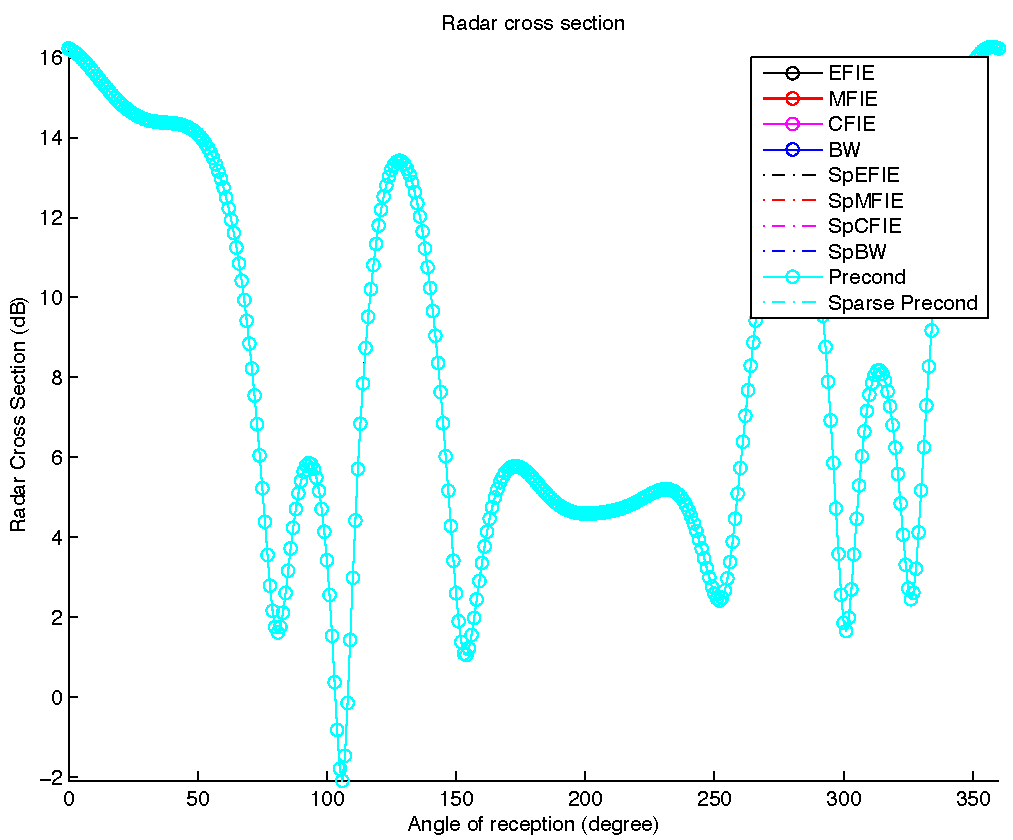
\includegraphics[width=0.45\textwidth]{matlab/fig_PlaneWaveDirichlet/RCS.pdf}}
\subfigure[History of convergence of the GMRES]{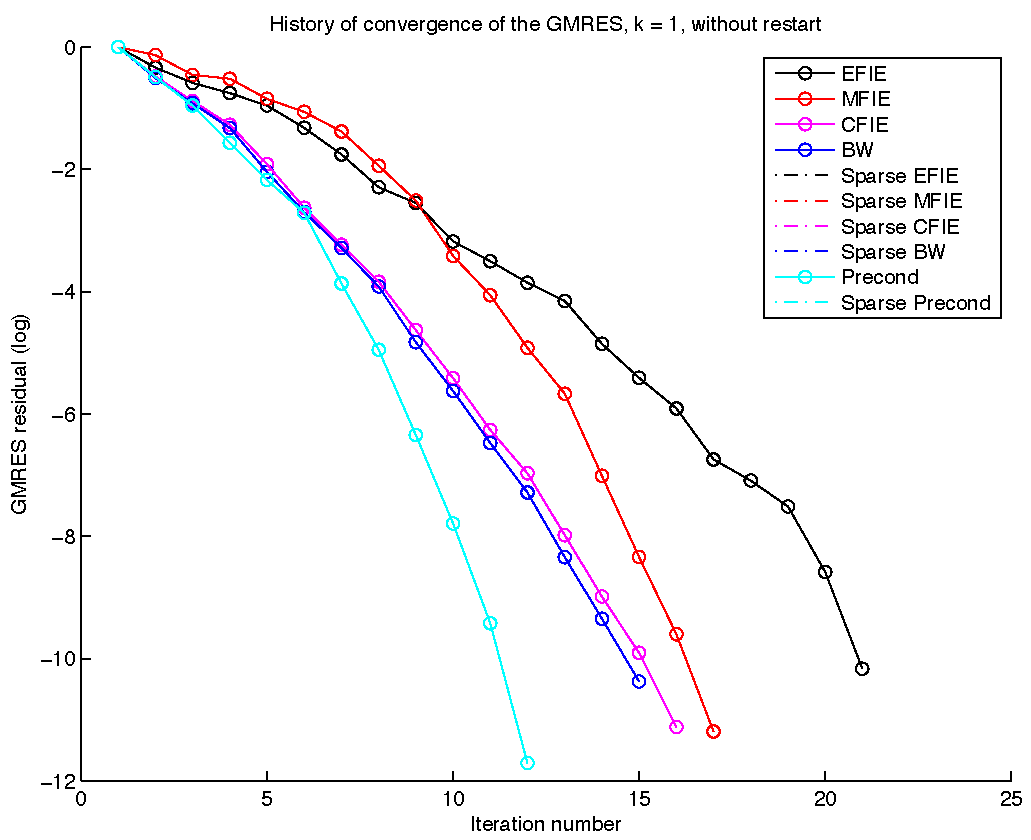
\includegraphics[width=0.45\textwidth]{matlab/fig_PlaneWaveDirichlet/gmres.pdf}}
\subfigure[Absolute value of the scattered field]{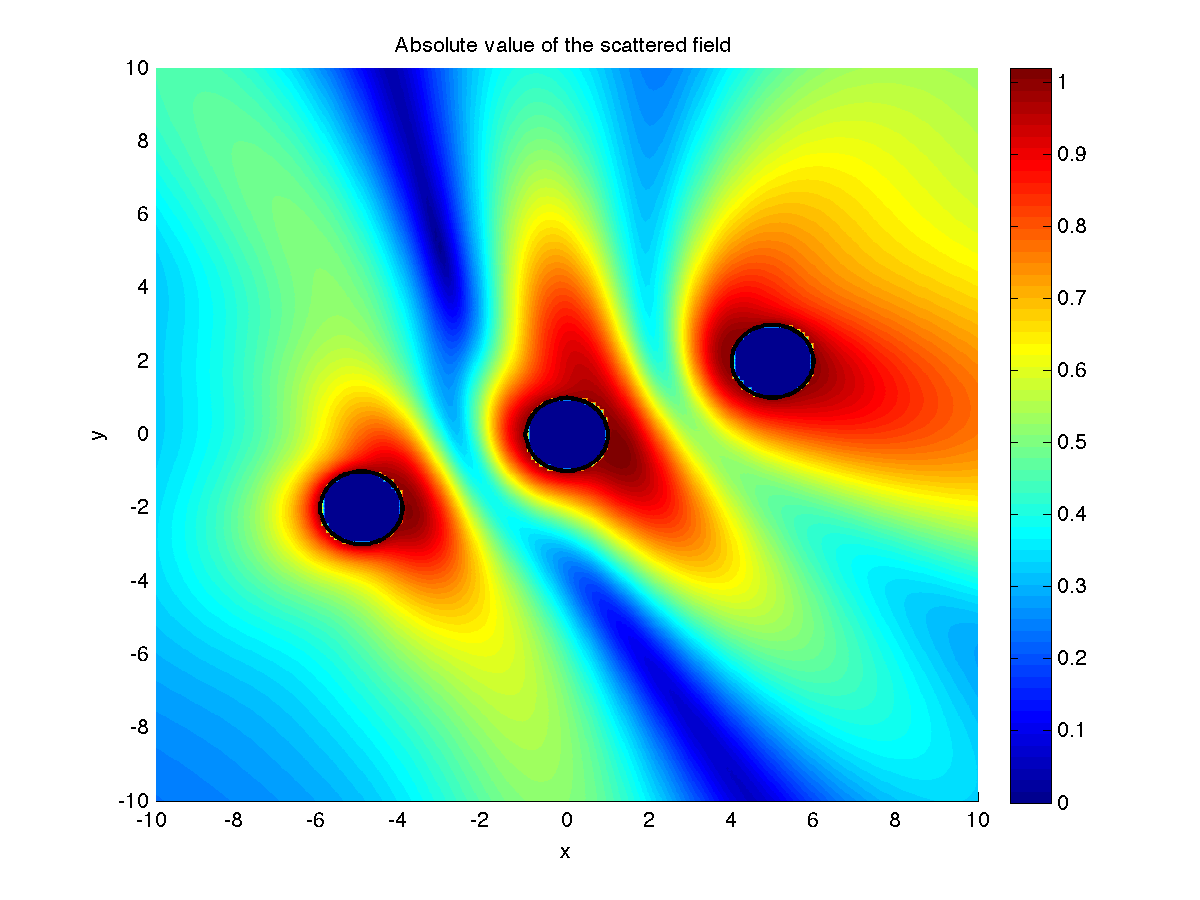
\includegraphics[width=0.45\textwidth]{matlab/fig_PlaneWaveDirichlet/u_abs.png}}
\subfigure[Absolute value of the total field]{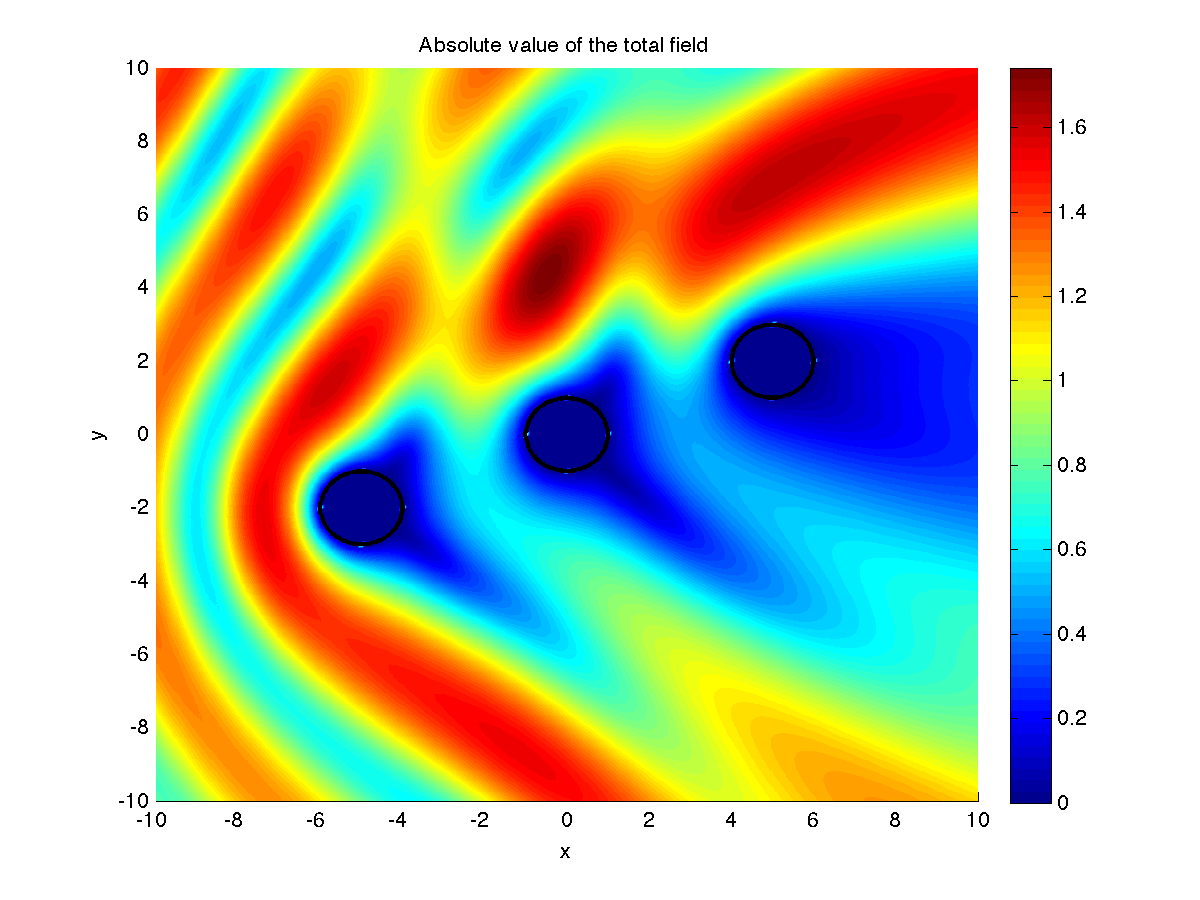
\includegraphics[width=0.45\textwidth]{matlab/fig_PlaneWaveDirichlet/utot_abs.png}}
\subfigure[Real part of the total field]{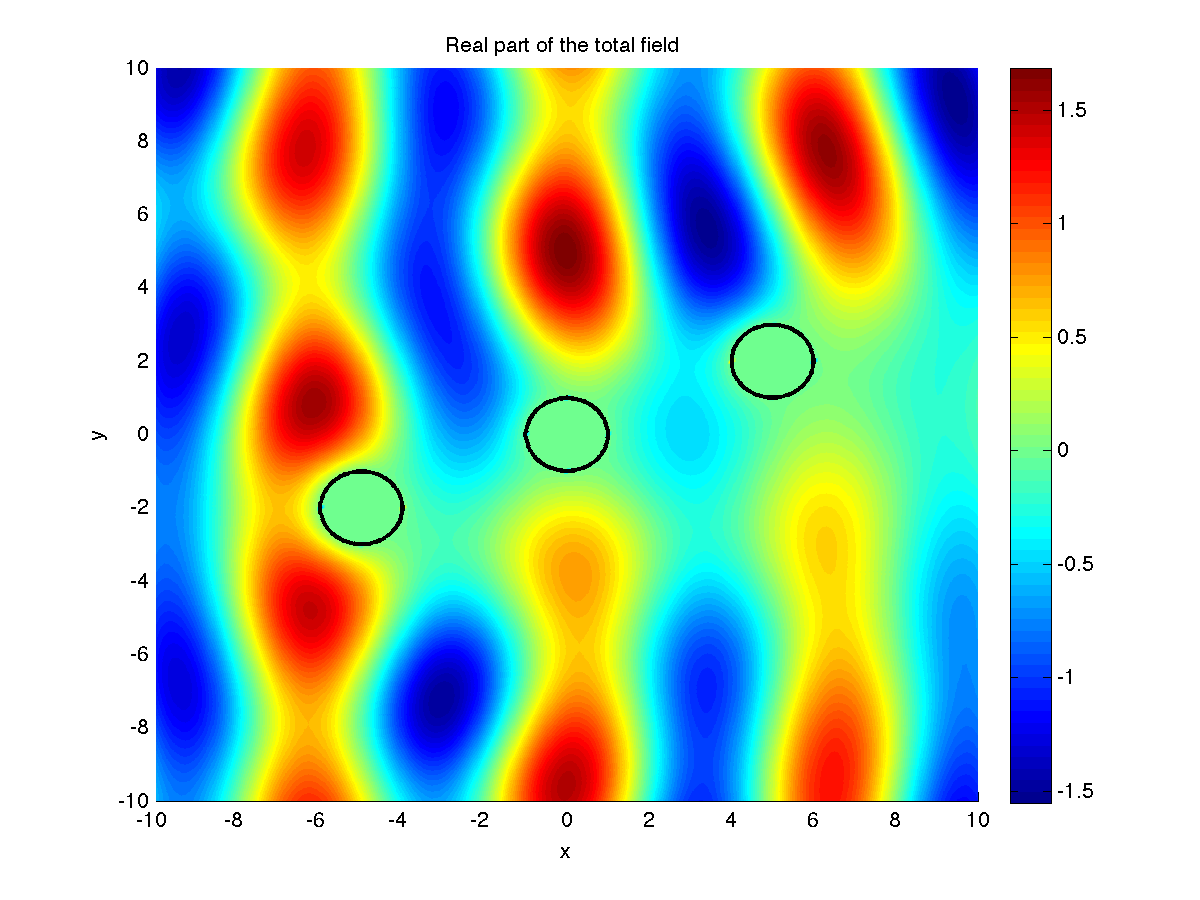
\includegraphics[width=0.45\textwidth]{matlab/fig_PlaneWaveDirichlet/utot_real.png}}
\caption{Different results for a Dirichlet problem and an incident plane wave solved using \mudiff. The first figure shows the three obstacles and the second one the radar cross section obtained for the different integral equation (all superimposed). The next figure (c) represents the GMRES history of convergence of the different integral equations. The figure (d) shows the absolute value of the scattered field, and the last two, (e) and (f), represent respectively the absolute value and the real part of the total field.}
\label{fig:exampleDirichlet}
\end{figure}

\subsection{Point source wave}

Our toolbox \mudiff also provides a right hand side derived from a wave emitted by a point source. To solve that kind of problem, the right hand side is built thanks to \PointSource and \DnPointSource instead of respectively \PlaneWave and \DnPlaneWave (there is currently no equivalent of \PlaneWavePrecond). For example, for the EFIE and a point source centered on $(-10,0)$, the right hand side must be computed as:
\begin{lstlisting}
XS = [-10; 0]; %location of the source (point source case)
%Right-hand side
Uinc = PointSource(O, a, M_modes, k, XS);
\end{lstlisting}
The other change appears in the post-processing when computing the total field on a grid. Indeed, the incident wave is different and \IncidentWaveOnGrid must get the right argument:
\begin{lstlisting}
UincOnMesh = IncidentWaveOnGrid(X, Y, k, 'PointSource', XS);
\end{lstlisting}

The rest of the code remains unchanged and the results obtained with a point source are shown on figure \ref{fig:exampleDirichletPS}.

\begin{figure}
\centering
\subfigure[Obstacles]{\includegraphics[width=0.45\textwidth]{matlab/fig_PointSourceDirichlet/obstacles.pdf}}
\subfigure[Radar cross section]{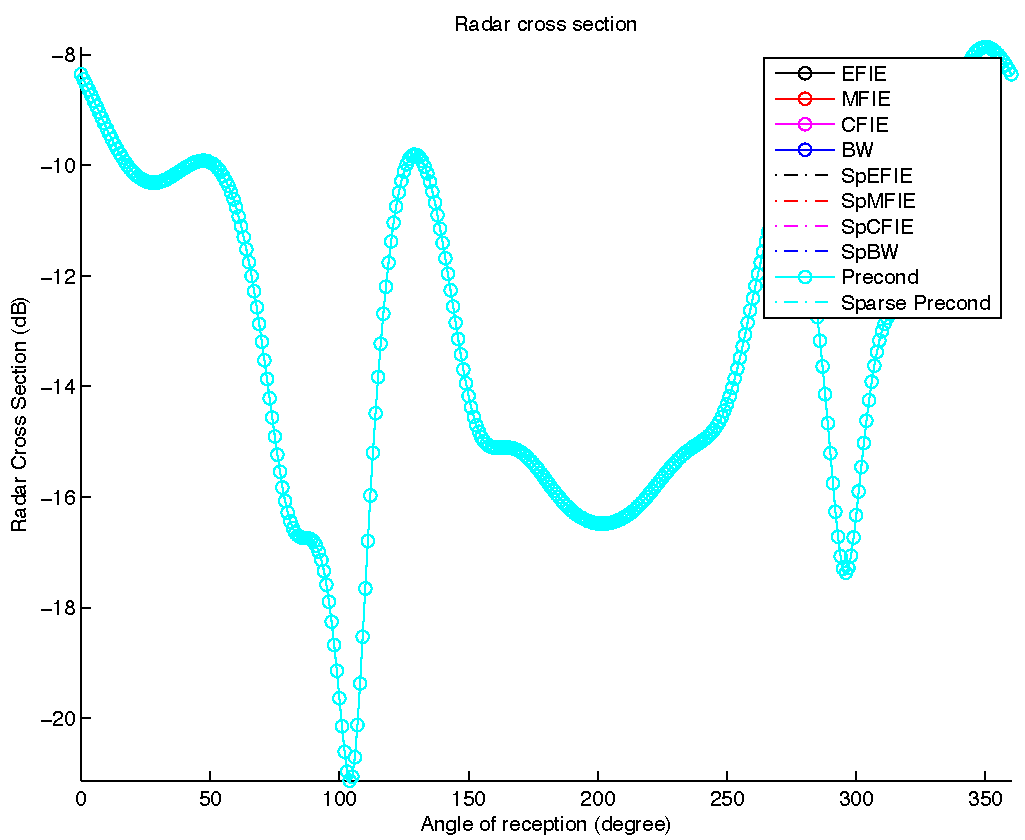
\includegraphics[width=0.45\textwidth]{matlab/fig_PointSourceDirichlet/RCS.pdf}}
\subfigure[History of convergence of the GMRES]{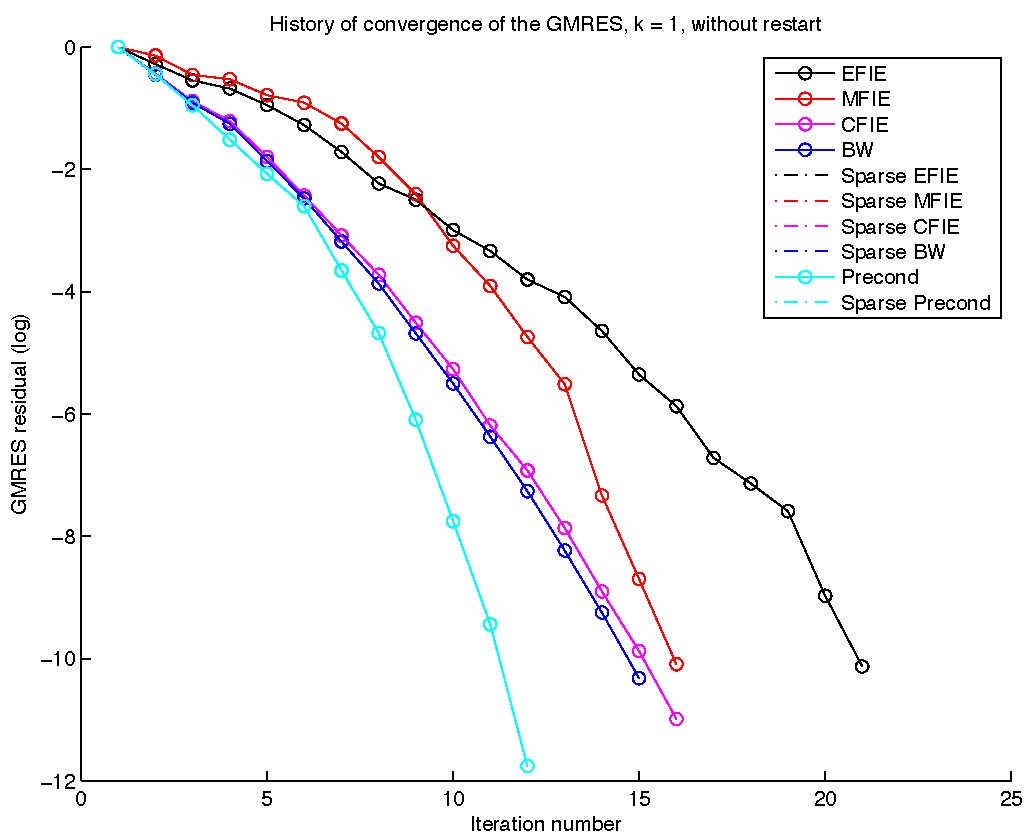
\includegraphics[width=0.45\textwidth]{matlab/fig_PointSourceDirichlet/gmres.pdf}}
\subfigure[Absolute value of the scattered field]{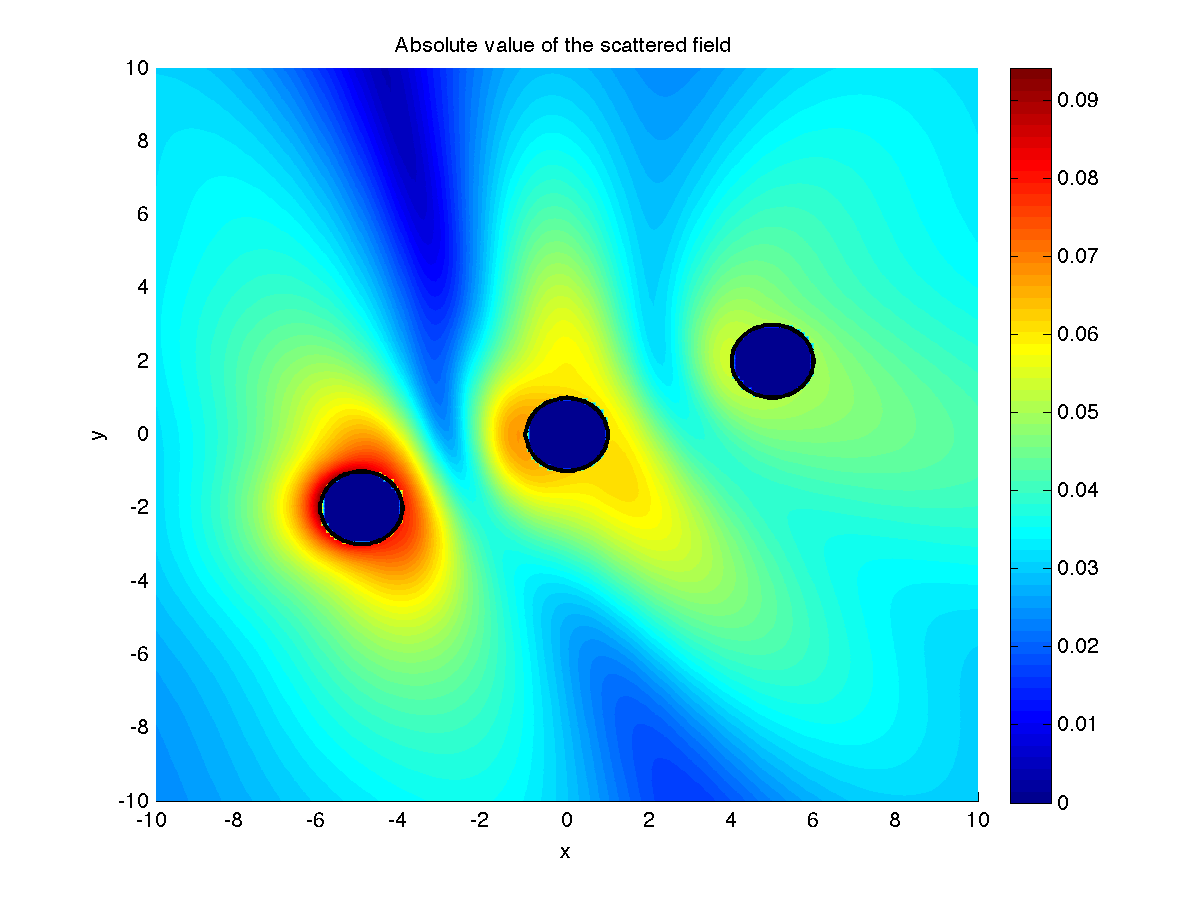
\includegraphics[width=0.45\textwidth]{matlab/fig_PointSourceDirichlet/u_abs.png}}
\subfigure[Absolute value of the total field]{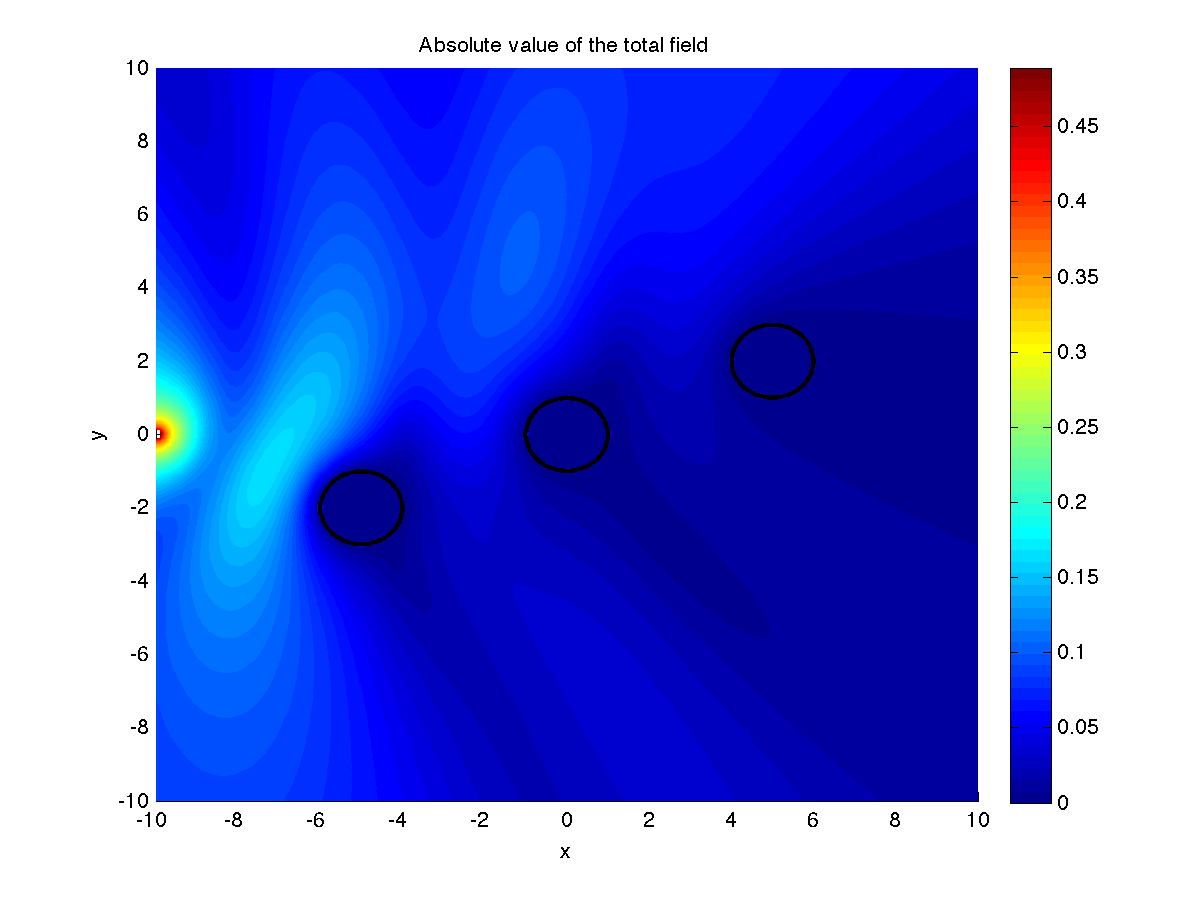
\includegraphics[width=0.45\textwidth]{matlab/fig_PointSourceDirichlet/utot_abs.png}}
\subfigure[Real part of the total field]{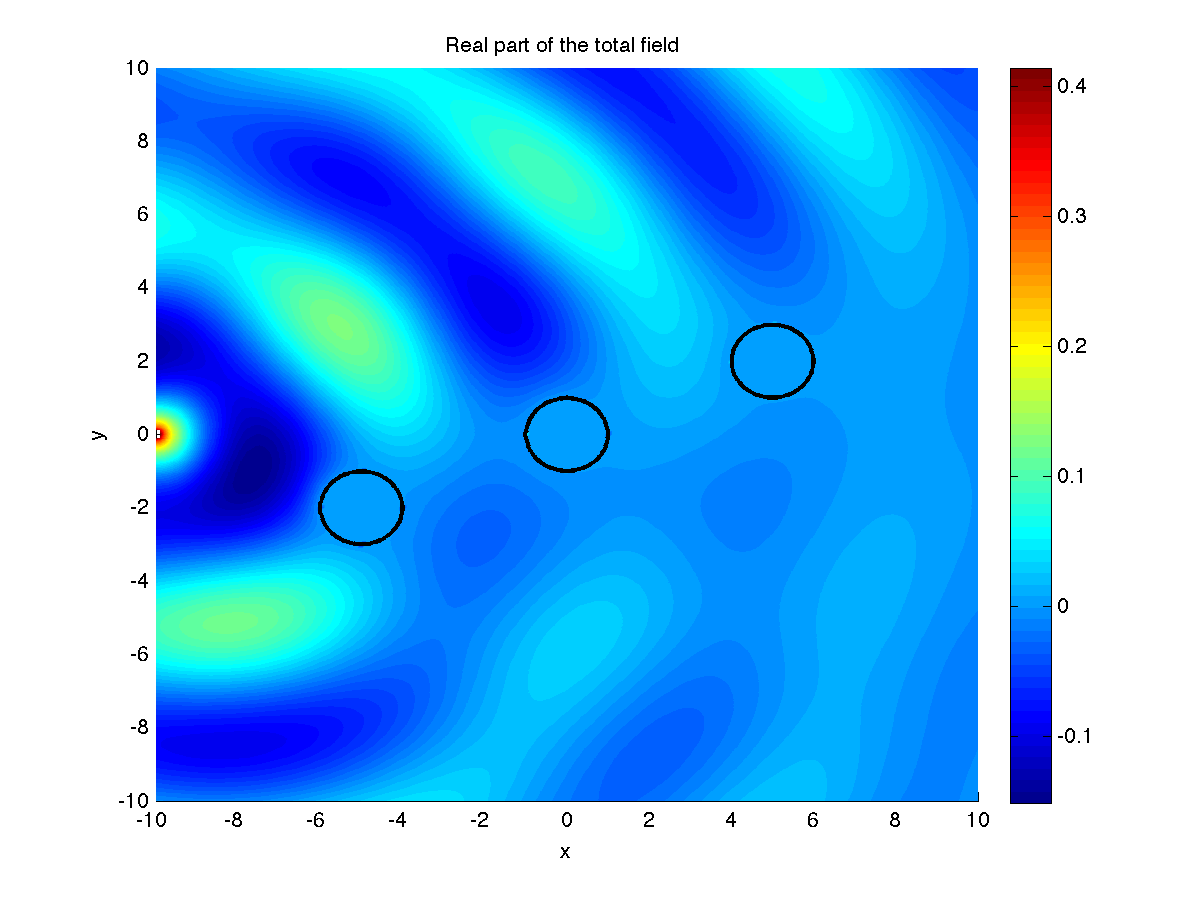
\includegraphics[width=0.45\textwidth]{matlab/fig_PointSourceDirichlet/utot_real.png}}
\caption{Different results for a Dirichlet problem for a wave emitted by a point source solved using \mudiff. The first two pictures show respectively the obstacles and the radar cross section, while the third one shows the GMRES history of convergence. The absolute value of the scattered field is presented on subfigure (d), and the total field on figures (e) (absolute value) and (f) (real part).}
\label{fig:exampleDirichletPS}
\end{figure}

%%%%%%%%%%%%%%%%%%%%%%%%%%%%%%%%%%%%%
\newpage
\section{The Neumann boundary-value problem}

Let us now consider the sound-hard scattering problem
$$
\left\{\begin{array}{r c l l}
(\Delta +k^2)u & = & 0, & \text{ in }\Omegaps,\\
\dn u & = & -\dn \uinc, & \text{ on }\Gamma,\\
\multicolumn{4}{l}{\qquad \qquad u \text{ outgoing}.}
\end{array}\right.
$$

An efficient solution to this problem is given for example by a preconditioned integral equation for sound-hard obstacles.
Here, we only present this solution but the extension to other kinds of integral equations is direct.
 The $\mu$-diff script is close to the one developed for the Dirichlet problem, only the two following functions must
  be modified: \PrecondDirichlet is replaced by \PrecondNeumann and the right-hand side \PlaneWavePrecond is now given by
   \DnPlaneWavePrecond. For the Neumann problem, the preconditioned boundary integral equation is based on the double-layer representation
$$
\begin{cases}
u = \Mop\lambda,\\
\widehat{D}^{-1} D \lambda = -\widehat{D}^{-1}\dn\uinc.
\end{cases}
$$
\begin{lstlisting}
% Three unit disks 
O = [-5, 0, 5; -2, 0, 2];
a = [1, 1, 1];
%Set the parameters...
k = 1; %wavenumber
beta_inc = 0; %incident angle
%Fourier series truncation parameter
M_modes = FourierTruncation(a, k, 'Min', 1);
%Right-hand side
DnUincPrecond = DnPlaneWavePrecond(O, a, M_modes, k, beta_inc);
%Matrix of the system (the two following lines are the same)
APrecond = PrecondNeumann(O, a, M_modes, k);
%Solving (here, direct)
lambda = APrecond \ DnUincPrecond;
\end{lstlisting}
\medskip

The post-processing is based on the double-layer potential (compared to Dirichlet, the modification is realized in the \RCS function, the
 last argument \code{[1,0]} is then replaced by  \code{[0,1]})
\begin{lstlisting}
%Scattering angles
theta_RCS = 0:360;
theta_RCS_rad = theta_RCS*2*pi/360;
%Radar Cross Section associated with the double-layer potential
myRCS = RCS(O, a, M_modes, k, theta_RCS_rad, lambda, [0,1]);
plot(theta_RCS, myRCS, 'k');
\end{lstlisting}

With the previous parameter, we obtain the result shown on figure \ref{fig:exampleNeumann} for an incident plane wave of direction $0$ and on figure \ref{fig:exampleNeumannPS} for a point source centered on $[-10,0]$. Only the case of the preconditioned integral equation has been shown.

\begin{figure}
\centering
\subfigure[Obstacles]{\includegraphics[width=0.45\textwidth]{matlab/fig_PlaneWaveNeumann/obstacles.pdf}}
\subfigure[Radar cross section]{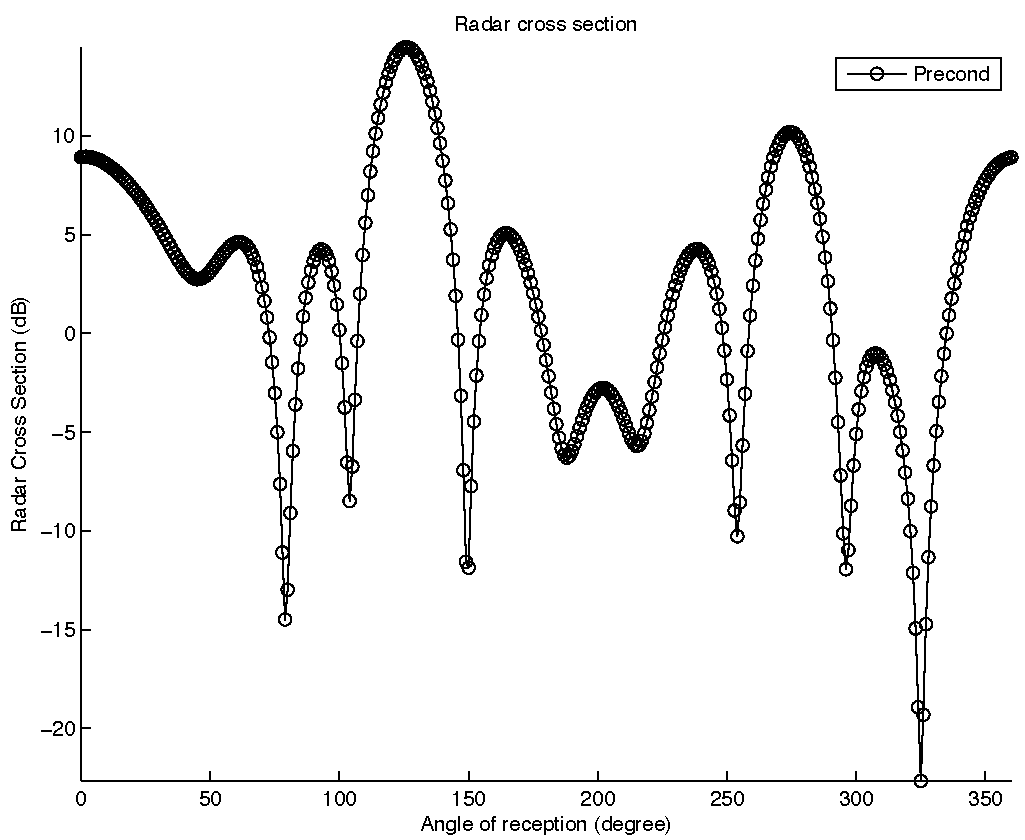
\includegraphics[width=0.45\textwidth]{matlab/fig_PlaneWaveNeumann/RCS.pdf}}
\subfigure[History of convergence of the GMRES]{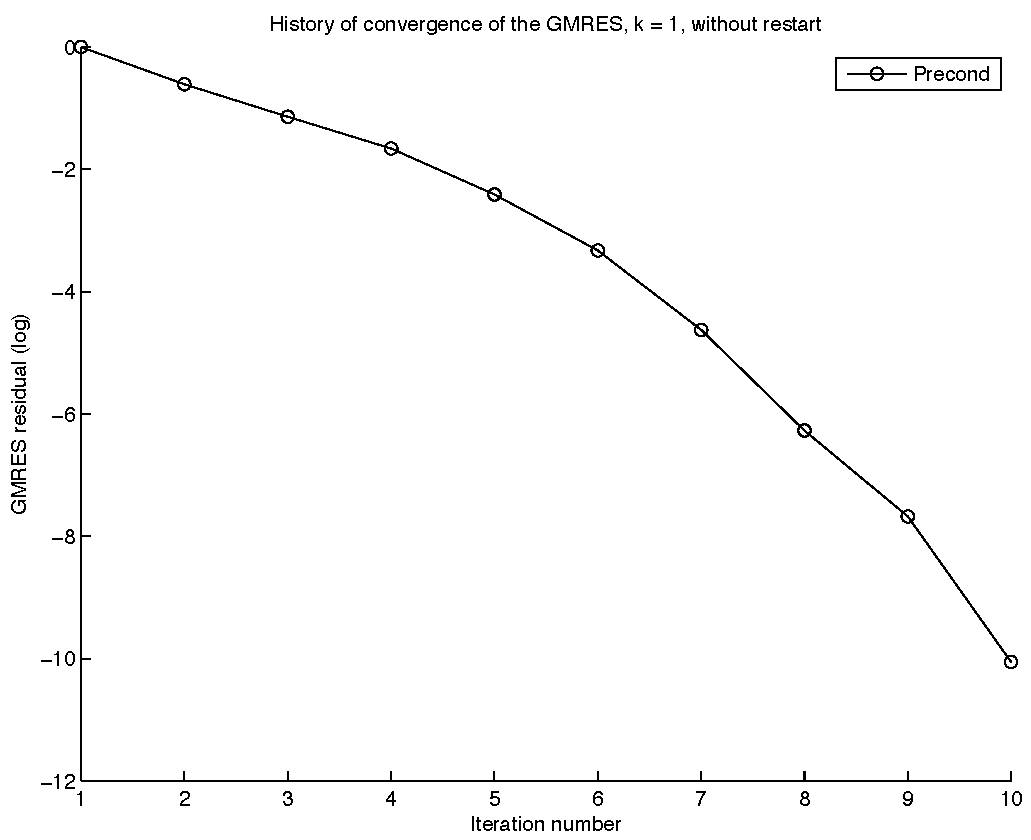
\includegraphics[width=0.45\textwidth]{matlab/fig_PlaneWaveNeumann/gmres.pdf}}
\subfigure[Absolute value of the scattered field]{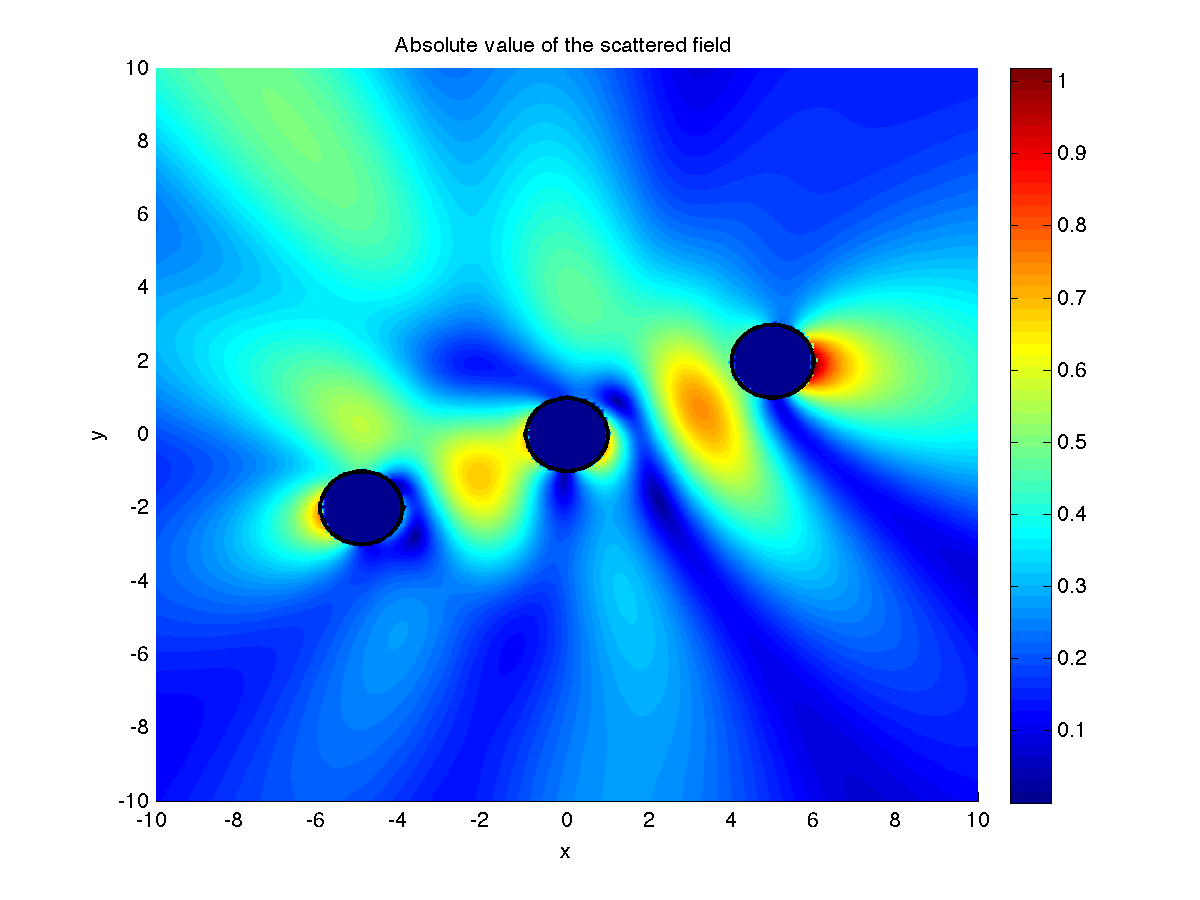
\includegraphics[width=0.45\textwidth]{matlab/fig_PlaneWaveNeumann/u_abs.png}}
\subfigure[Absolute value of the total field]{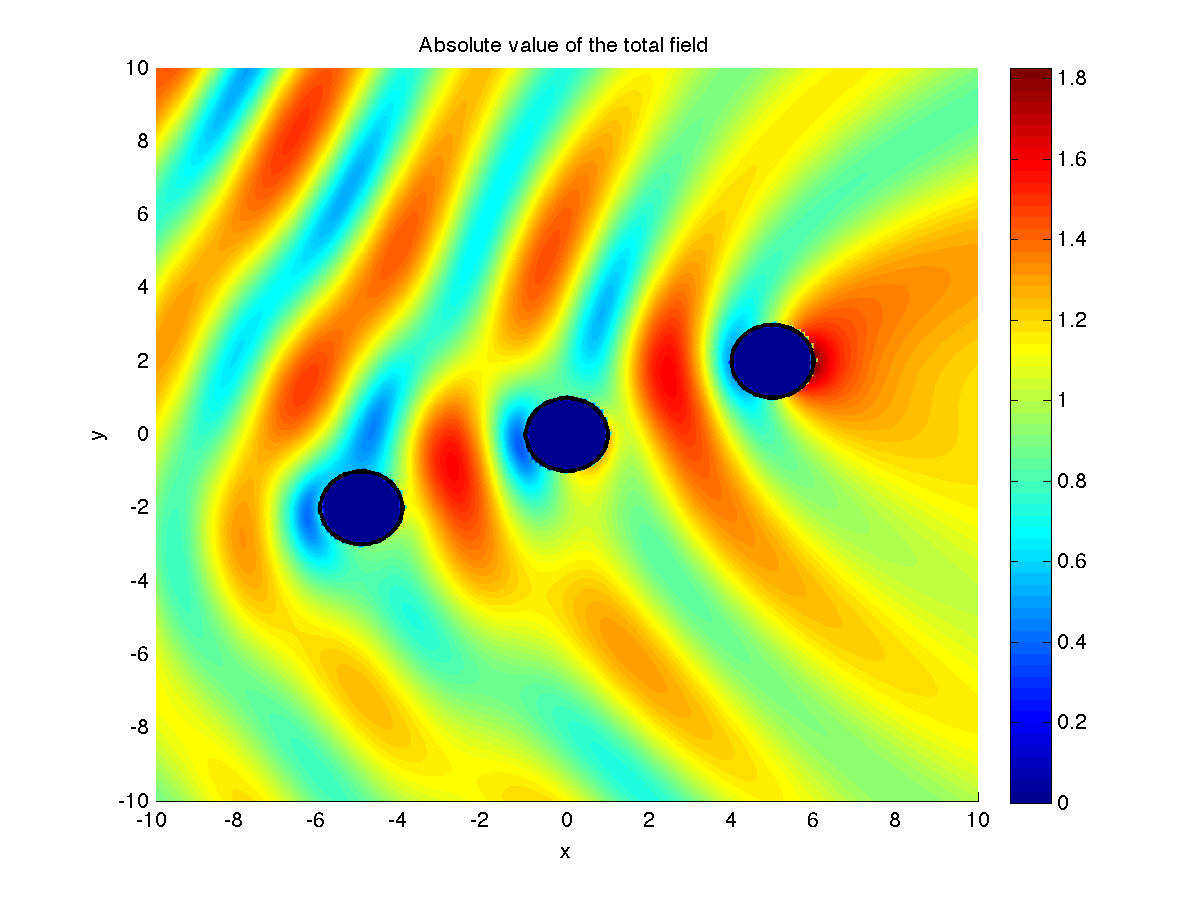
\includegraphics[width=0.45\textwidth]{matlab/fig_PlaneWaveNeumann/utot_abs.png}}
\subfigure[Real part of the total field]{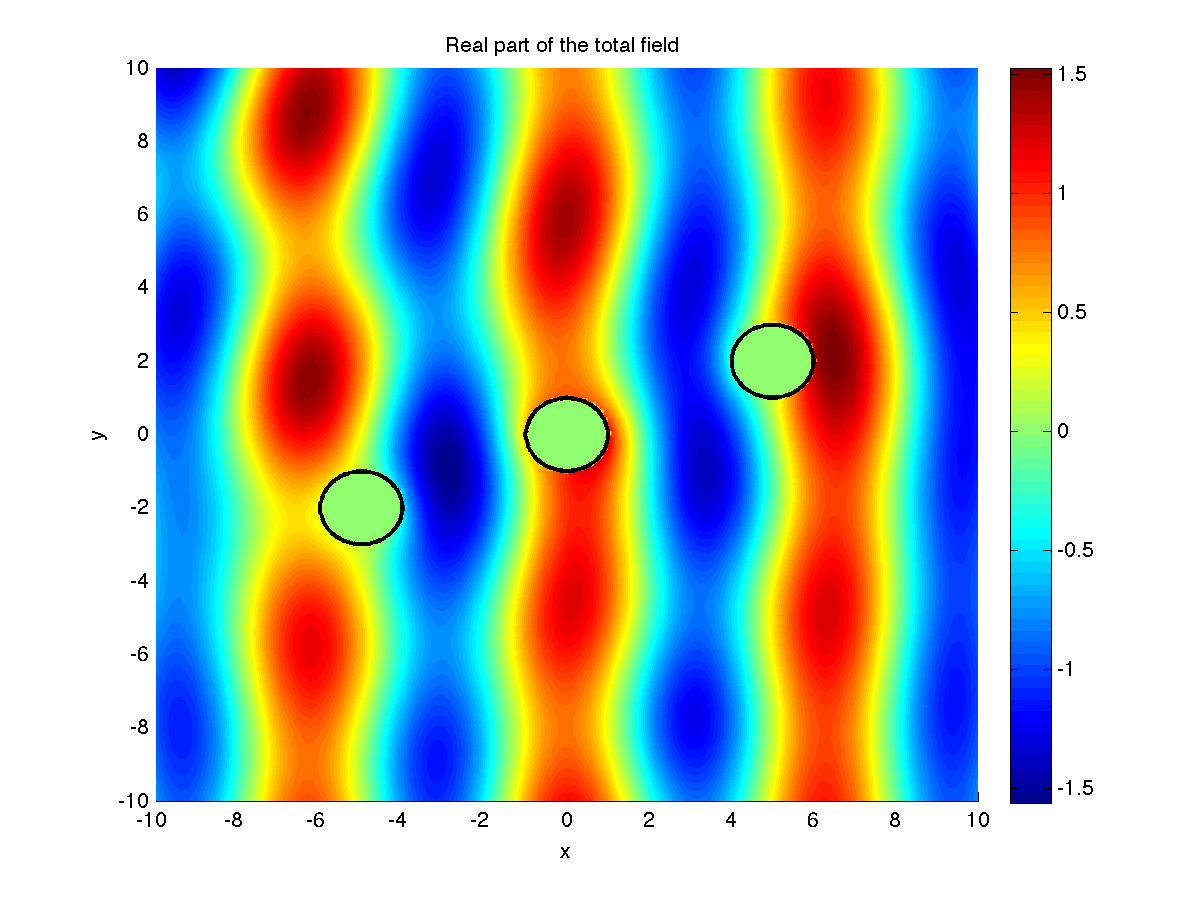
\includegraphics[width=0.45\textwidth]{matlab/fig_PlaneWaveNeumann/utot_real.png}}
\caption{Neumann boundary value problem with an incident plane wave of direction $0$, solved using (only) the single scattering preconditioned integral equation. The three first figures show respectively: the obstacles, the radar cross section, the history of convergence of the GMRES. The three last, (d) to (f), present the absolute value of the scattered field, the absolute and real part of the total field.}
\label{fig:exampleNeumann}
\end{figure}


\begin{figure}
\centering
\subfigure[Obstacles]{\includegraphics[width=0.45\textwidth]{matlab/fig_PointSourceNeumann/obstacles.pdf}}
\subfigure[Radar cross section]{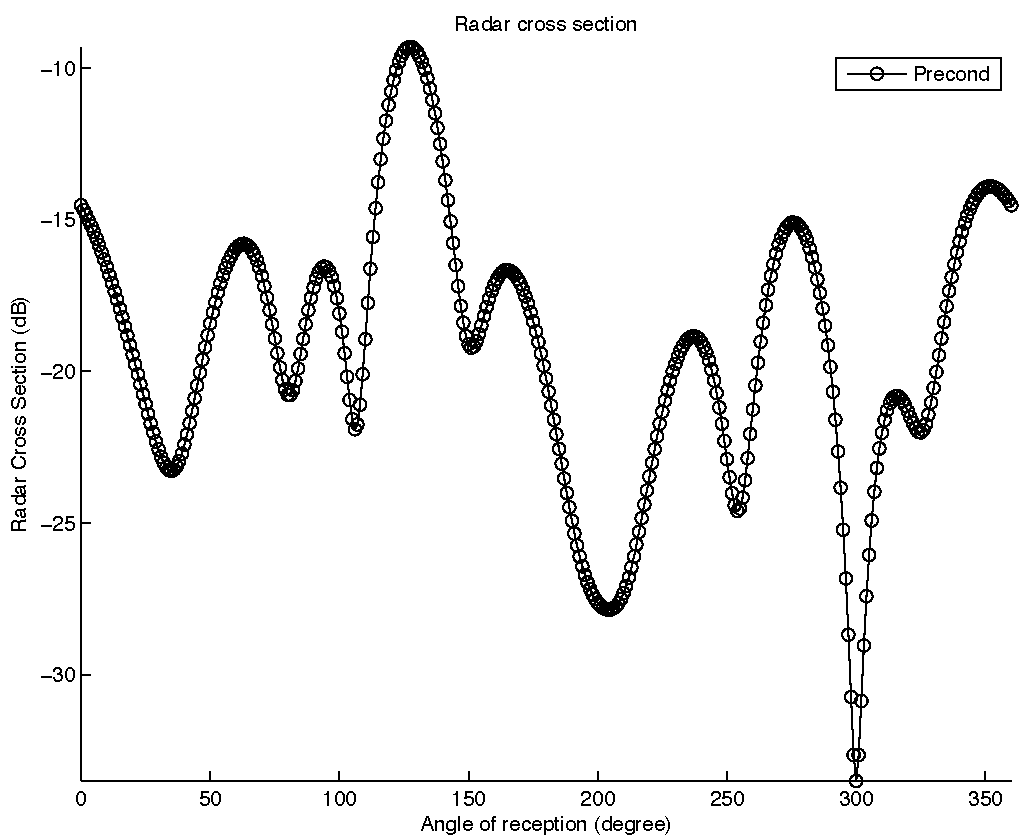
\includegraphics[width=0.45\textwidth]{matlab/fig_PointSourceNeumann/RCS.pdf}}
\subfigure[History of convergence of the GMRES]{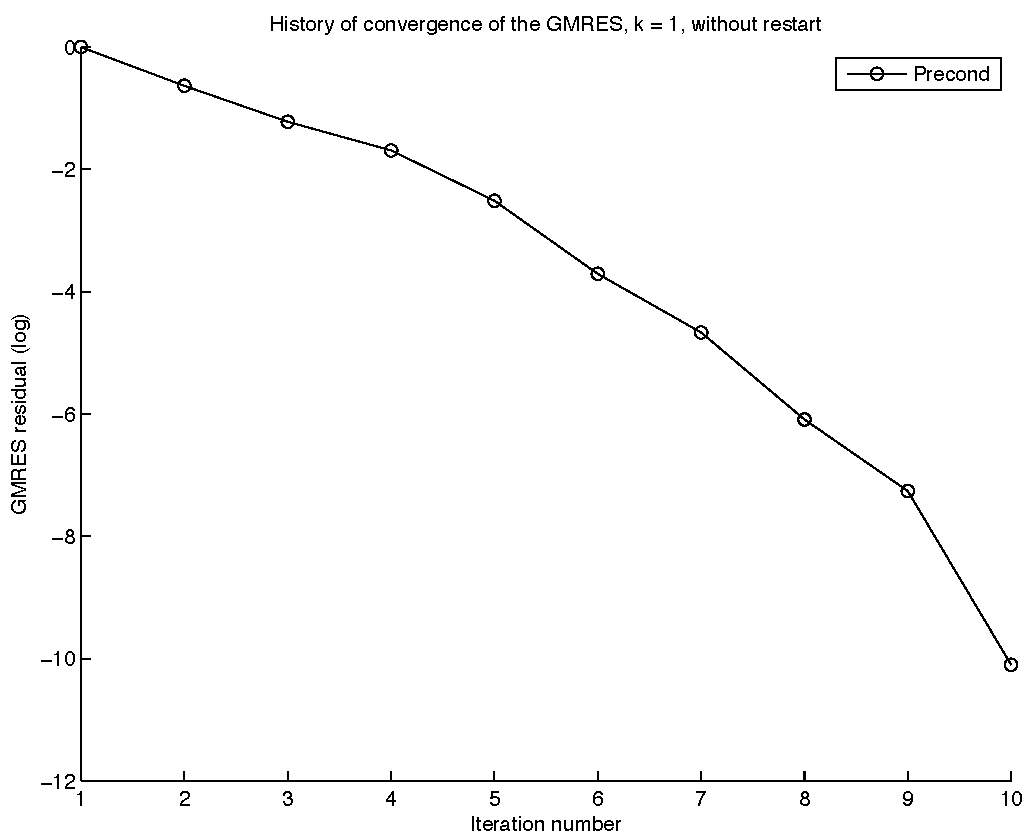
\includegraphics[width=0.45\textwidth]{matlab/fig_PointSourceNeumann/gmres.pdf}}
\subfigure[Absolute value of the scattered field]{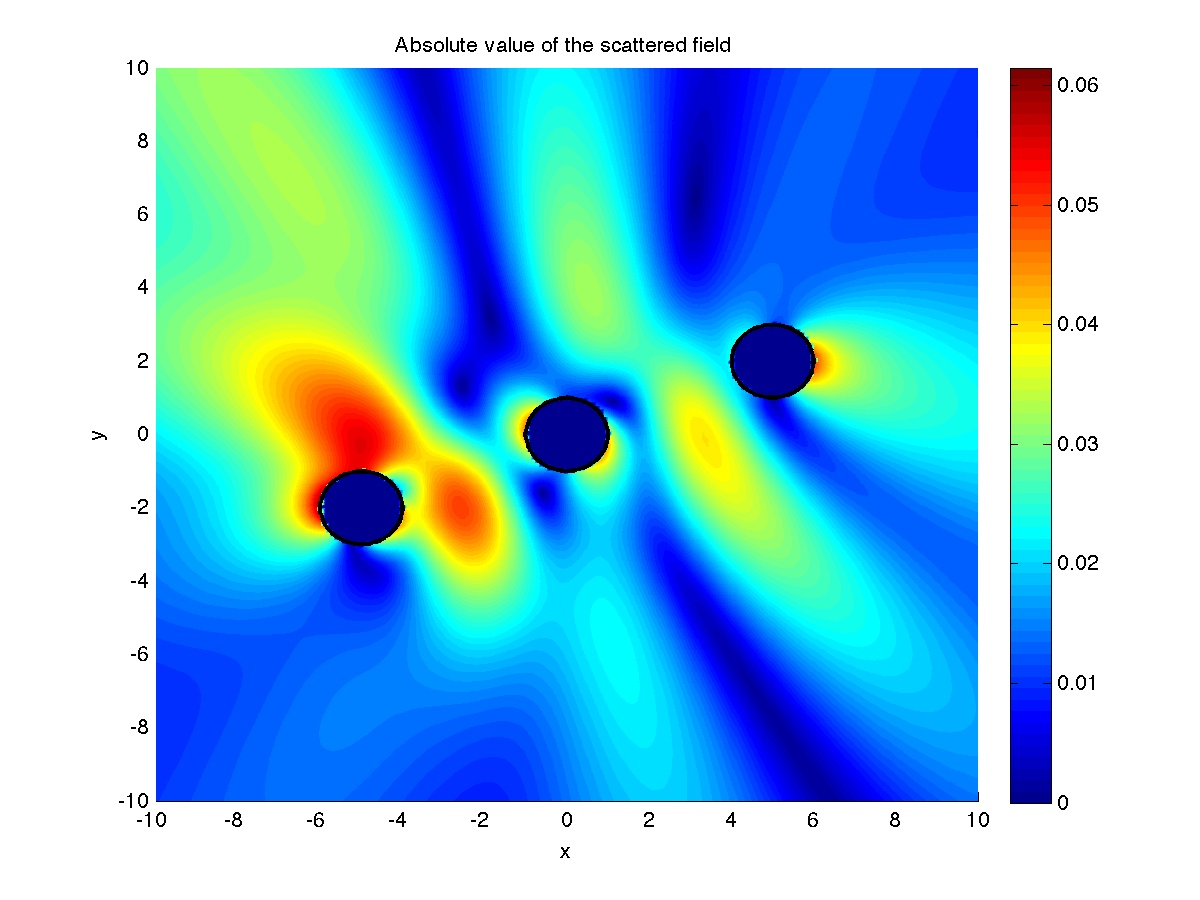
\includegraphics[width=0.45\textwidth]{matlab/fig_PointSourceNeumann/u_abs.png}}
\subfigure[Absolute value of the total field]{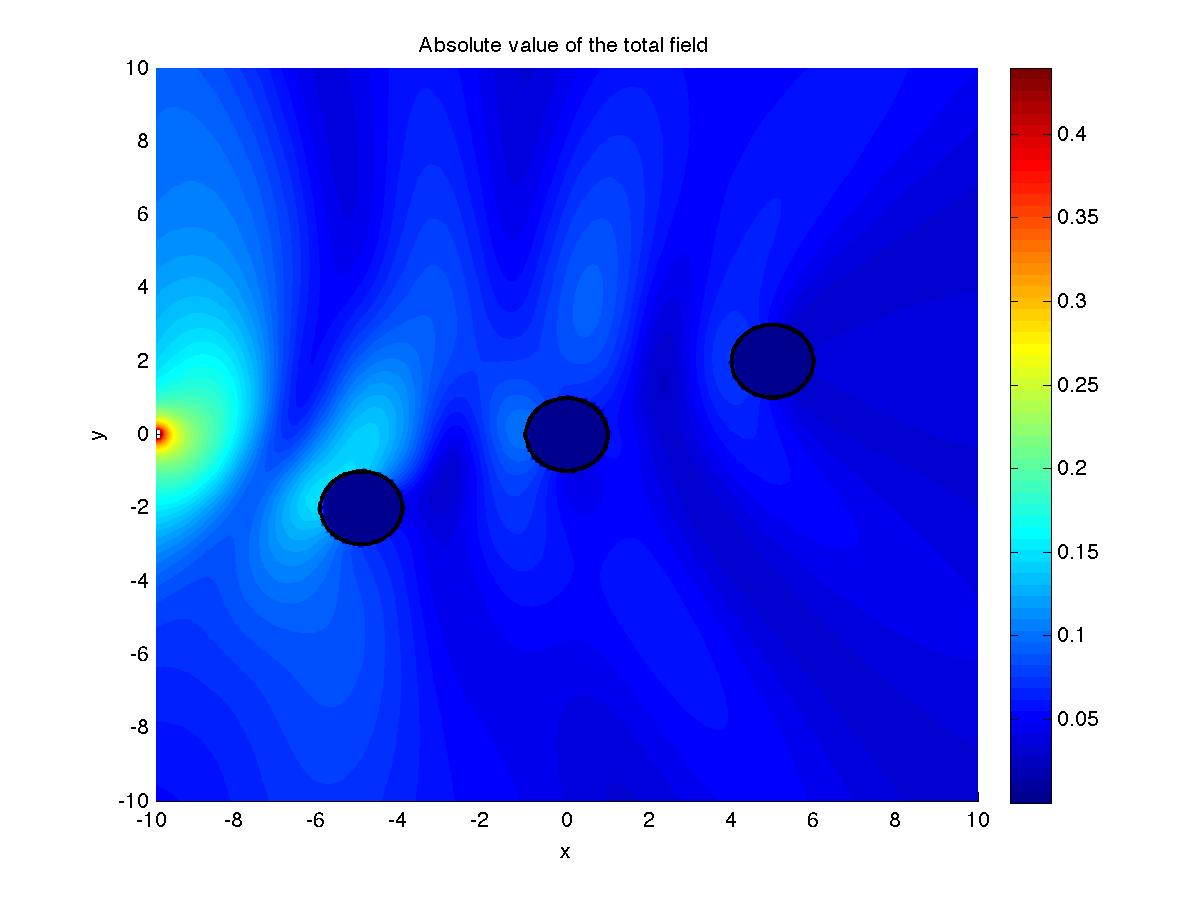
\includegraphics[width=0.45\textwidth]{matlab/fig_PointSourceNeumann/utot_abs.png}}
\subfigure[Real part of the total field]{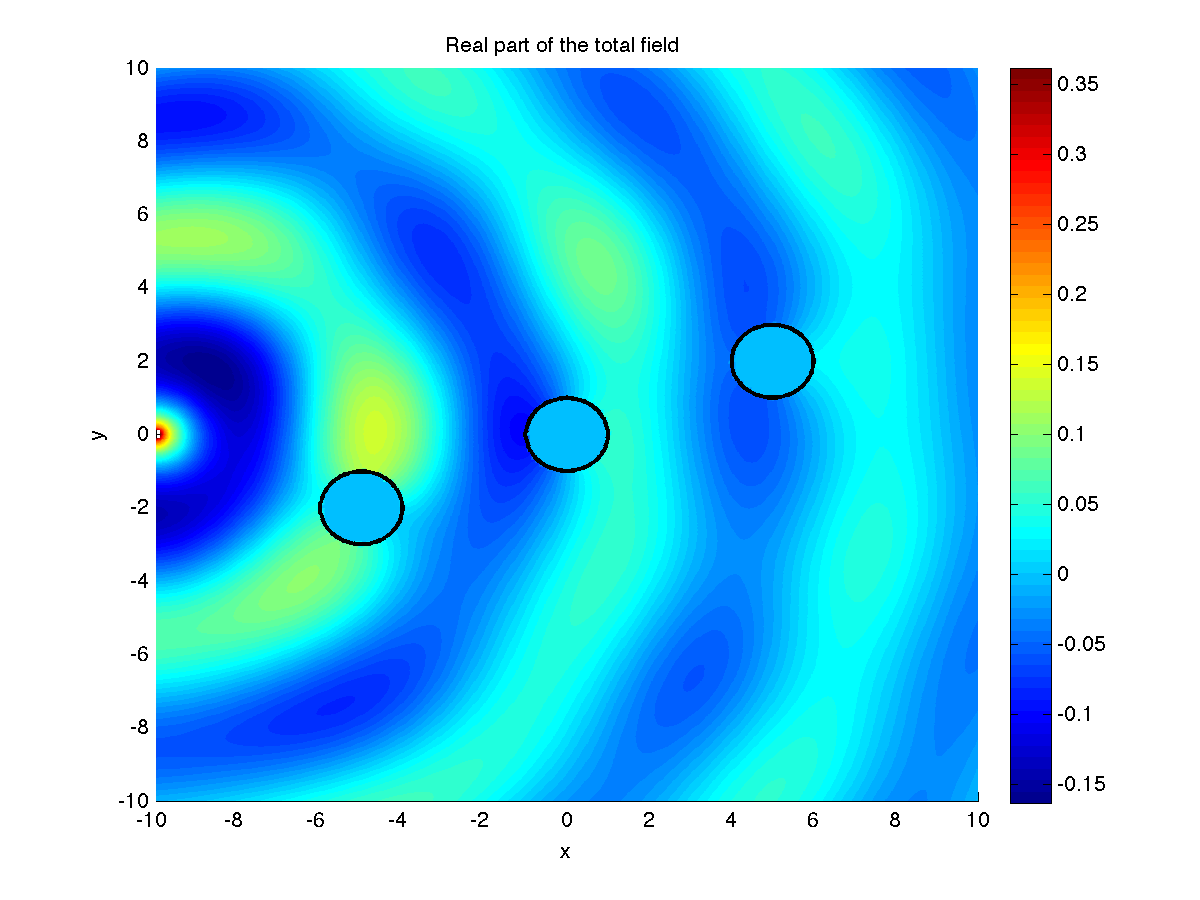
\includegraphics[width=0.45\textwidth]{matlab/fig_PointSourceNeumann/utot_real.png}}
\caption{Neumann boundary value problem with a point source emitter solved using the single scattering preconditioned integral equation. In the respective order is shown: the obstacles, the radar cross section, the history of convergence of the GMRES and then, the absolute value of the scattered field, the absolute and real part of the total field.}
\label{fig:exampleNeumannPS}
\end{figure}


%%%%%%%%%%%%%%%%%%%%%%%%%%%%%%%%%%%%%%%%%%%%%%
\newpage
\section{Mixing Dirichlet and Neumann boundary conditions}

Let us consider the following situation where we mix Dirichlet and Neumann boundary conditions. The scatterer is composed of
 $M_D$ sound-soft and  $M_N = M-M_D$ sound-hard obstacles, leading to the scattering problem
$$
\left\{\begin{array}{r c l l}
(\Delta +k^2)u & = & 0, & \text{ in }\Omegaps,\\
u & = & -\uinc, & \text{ on }\Gamma_p,\quad p=1,\ldots, M_D,\\
\dn u & = & -\dn \uinc, & \text{ on }\Gamma_p,\quad p=M_D+1,\ldots, M,\\
\multicolumn{4}{l}{\qquad \qquad u \text{ outgoing}.}
\end{array}\right.
$$
For this problem, the  preconditioned integral is not directly available. We can apply a Combined Field Integral Equation for the mixed problem
 (see equation (\ref{eq:CFIEMixte2})) and written as $$(\frac{I}{2} +A)\varphi = b,$$ where
  the matrix $A$ is
  given by  (\ref{eq:CFIEMixteApq}). We have
$$
A(p,q) = 
\begin{cases}
(1-\alpha) N^{p,q} + \alpha\eta L^{p,q}, & \text{ if } q \leq M_D,\\
(1-\alpha) D^{p,q} + \alpha\eta M^{p,q}, & \text{ if } q > M_D.\\
\end{cases}
$$
The  matrix is particularly easy to build  with \mudiff thanks to the frontal function \IntegralOperator. To this end, two
 three-dimensional arrays, \code{Assembling} and \code{Weight}, are built such that
$$
\code{Assembling}(:, p,q) = 
\begin{cases}
[4,2], & \text{ if } q \leq M_D,\\
[5,3], & \text{ if } q > M_D,
\end{cases}\qquad\text{and}\qquad
\code{Weight}(:, p,q) = [(1-\alpha), \alpha\eta].
$$
The indices in \code{Assembling} corresponds to the indices of the boundary integral operators ($2=L^{p,q}$, $3=M^{p,q}$, $4=N^{p,q}$, $5=D^{p,q}$). The assembling process is realized by \IntegralOperator.
\begin{lstlisting}
% Two Dirichlet obstacles (unit diks)
OD = [-5, -5; -5, 5];
aD = [1, 1];
N_scatD = length(aD);
% Two Neumann obstacles (unit diks)
ON = [5, 5; -5, 5];
aN = [1, 1];
N_scatN = length(aN);
%All obstacles
O = [OD, ON];
a = [aD, aN];
N_scat = N_scatD + N_scatN;
%Set the parameters...
k = 1; %wavenumber
beta_inc = 0; %incident angle
%Fourier series truncation parameter (Dirichlet, Neumann, All)
M_modesD = FourierTruncation(aD, k, 'Min', 1);
M_modesN = FourierTruncation(aN, k, 'Min', 1);
M_modes = [M_modesD, M_modesN];
%Right-hand side
Uinc = DnPlaneWave(O, a, M_modes, k, beta_inc);
DnUinc = DnPlaneWave(O, a, M_modes, k, beta_inc);
B = alpha*eta*Uinc + (1-alpha)*DnUinc;
%% Assembling
Assembling = zeros(2, N_scat, N_scat);
Weight = zeros(2, N_scat, N_scat);
for p=1:N_scatD
	for q=1:N_scat
		Assembling(:,p,q) = [4;2]; %4=N, 2=L
		Weight(:,p,q) = [1-alpha; alpha*eta];
	end
end
for p=N_scatD+1:N_scat
	for q=1:N_scat
		Assembling(:,p,q) = [5;3];%5=D, 3=M
		Weight(:,p,q) = [1-alpha; alpha*eta];
	end
end
%Common function
A = IntegralOperator(O, a, M_modes, k, Assembling, Weight);
%Solving (here, direct)
density = A \ B;
\end{lstlisting}
\medskip

The post-processing is then done by specifying to \mudiff how the density must be used: for the first $M_D$ obstacles, a single-layer potential is used,
while for the others, a double-layer potential is required. The \RCS function can simply do that. It just needs an array \code{TypeOfOp} of size
 $\code{N\_scat}\times 2$ such that
$$
\code{TypeOfOp}(p,:) = \begin{cases}
[1,0], &\text{ if } p \leq M_D,\\
[0,1], &\text{ if } p > M_D.
\end{cases}
$$
In a \mudiff script, this  means ``Apply the single-layer potential (multiplied by $1$) for the first $M_D$ part of the density and a double-layer potential
 (multiplied by $1$) for the others''.
\begin{lstlisting}
%Preparing TypeOfOp
TypeOfOp = zeros(N_scat, 2);
for p =1:N_scat
	if(p <= N_scatD)
		TypeOfOp(p,1) = 1;
	else
		TypeOfOp(p,2) = 1;
	end
end
%Scattering angles
theta_RCS = 0:360;
theta_RCS_rad = theta_RCS*2*pi/360;
%Radar Cross Section computation
myRCS = RCS(O, a, M_modes, k, theta_RCS_rad, density, TypeOfOp);
plot(theta_RCS, myRCS, 'k');
\end{lstlisting}


%%%%%%%%%%%%%%%%%%%%%%%%%
\newpage
\section{Penetrable case}

\subsection{Integral equation}
Let us now consider the case of penetrable obstacles, with a frequency $k^-_p$ (possibly different) in each scatterer $\Omegamp$, for $p=1,\ldots,M$. The problem then reads as:
$$
\left\{\begin{array}{r c l l}
(\Delta +(k^+)^2)u^+ & = & 0, & \text{ in }\Omegaps,\\
(\Delta +(k^-)^2)u^- & = & 0, & \text{ in }\Omegam,\\
u^+ - u^- & = & -\uinc, & \text{ on }\Gamma,\\
\dn u^+ -\dn u^- & = & -\dn \uinc, & \text{ on }\Gamma,\\
\multicolumn{4}{l}{\qquad \qquad u^+ \text{ outgoing},}
\end{array}\right.
$$
where $k^-|_{\Omegam_p} = k^-_p$.  Solving this problem can be done thanks to the integral equation presented in section \ref{eq:SystPenet} where the interior total field $\um$ (equal also to the total field) and the exterior scattered field $\ups$ are represented as a single-layer potential:
$$
\begin{cases}
\dsp \ups(\xx)  = \Lop^+\rhops(\xx) = \int_\Gamma G^+(\xx,\yy)\rhops(\yy)\;\dd\yy & \text{ in }\Omegaps,\\
\dsp \um(\xx)  = \Lop^-\rhomi(\xx) = \int_\Gamma G^-(\xx,\yy)\rhomi(\yy)\;\dd\yy & \text{ in }\Omegam,
\end{cases}
$$
The associated integral equation (\ref{eq:SystPenet}) is recalled to be
$$
\left(\begin{array}{c c}
\dsp L^+ & -L^-\\
\dsp -\frac{I}{2} + N^+ & \dsp -\frac{I}{2} - N^-
\end{array}\right)
\left(\begin{array}{c}
\rhops\\
\rhomi
\end{array}\right)
=
\left(\begin{array}{c}
-\uinc|_\Gamma\\
-\dn\uinc|_\Gamma
\end{array}\right).
$$

\subsection{A more complex geometry}

As already explained in \S\ref{sec:placementObstacles}, \mudiff also proposes some tools to place the obstacles and in a particular order, leading to original geometry, as the one shown previously on figure \ref{fig:removeDisks} and treated here (see \ref{fig:exwaveguidea}). The geometry is composed by a periodic placement of $11 \times 11$ unit disks, separated by a distance equal to $1$ with an empty middle line and middle column, leading to, in fact, $10 \times 10 = 100$ obstacles. Below is recalled the code to obtain this geometry:

\begin{lstlisting}
bx = 3; by = 3;
Nx = 11; Ny = 11;
O = RectangularLattice(bx, by, Nx, Ny, 'Centered', [0, 0]);
a = ones(1, size(O, 2));
[O, a] = RemoveDisk(O, a, 'X', 0, 'Y', 0);
N_scat = size(O,2);
\end{lstlisting}

\subsection{Writing and solving the BIE using \mudiff}

Let us solve the problem using a dense storage and first write the matrix of the system, which consists in assembling the different operator into a larger matrix:

\begin{lstlisting}
Splus = SingleLayer(O, a, M_modes, k); 
Sminus = IntegralOperator(O, a, M_modes, k_int, 2*eye(N_scat,N_scat));
Nplus = DnSingleLayer(O, a, M_modes, k);
Nminus = IntegralOperator(O, a, M_modes, k_int, 4*eye(N_scat,N_scat));
Identity = eye(size(Nplus));
% Boundary integral operator
A = [Splus, -Sminus; -0.5*Identity + Nplus, -(0.5*Identity + Nminus)];
%cleaning memory
clear Splus Sminus Nplus Nminus Identity mu_matrix;
\end{lstlisting}

Second, we need to introduce the right hand side (here a point source):

\begin{lstlisting}
Uinc = PointSource(O, a, M_modes, k, XS);
DnUinc = DnPointSource(O, a, M_modes, k, XS);
[B] = [Uinc;DnUinc];
clear Uinc DnUinc;
\end{lstlisting}
Finally, we solve the system, here using a direct solver. The two densities $\rho^+$ and $\rho^-$ are here also extracted to simplify:
\begin{lstlisting}
rho = A\B;
%% Extracting the "exterior" and "interior" densities
rho_plus = rho(1:sum_modes);
rho_minus = rho(sum_modes+1:end);
clear rho;
\end{lstlisting}

\subsection{Post-processing}

\subsubsection{Radar cross section}

We compute now the radar cross section, which is  based on the (exterior) single-layer potential:
\begin{lstlisting}
theta_RCS = 0:360;
theta_RCS_rad = theta_RCS*2*pi/360;
R = RCS(O, a, M_modes, k, theta_RCS_rad, rho_plus, [1,0]);
\end{lstlisting}
The radar cross section is shown on figure \ref{fig:exwaveguideb}. 

\subsubsection{Near field}

Let us now compute  the near-fields by first building the grid:
\begin{lstlisting}
XX = [-20:0.1:20];
YY = [-20:0.1:20];
[X,Y] = meshgrid(XX,YY);
\end{lstlisting}
And second, we compute the single-layer potentials, external and internal:
\begin{lstlisting}
%%Potentials
Ue = ExternalPotential(X, Y, O, a, M_modes, k, rho_plus, [1,0]);
Ui = InternalPotential(X, Y, O, a, M_modes, k_int, rho_minus, [1,0], 'OnBoundary', 1);
U = Ue + Ui;
\end{lstlisting}
The quantity \code{U} is the scattered field outside the obstacles and the total field inside in the obstacles. The option \code{OnBoundary} is set to compute the potential also on the boundary, in case there is some points of the grid on it. To get the total field, we need to add the incident wave to \code{U}, outside the obstacles:
\begin{lstlisting}
UincOnMesh = IncidentWaveOnGrid(X, Y, k, 'PointSource', XS);
Matrix_Not_Obstacles = (MaskMatrixObstacles(X, Y, O, a) == 0);
UincOnMesh = UincOnMesh.*Matrix_Not_Obstacles;
U_tot = U + UincOnMesh;
\end{lstlisting}
The near-fields are now fully computed and can be displayed. Figure \ref{fig:exwaveguided} represents the absolute value of the total field, and \ref{fig:exwaveguidee} and \ref{fig:exwaveguidef} its real and imaginary part.

\begin{figure}
\centering
\subfigure[Obstacles]{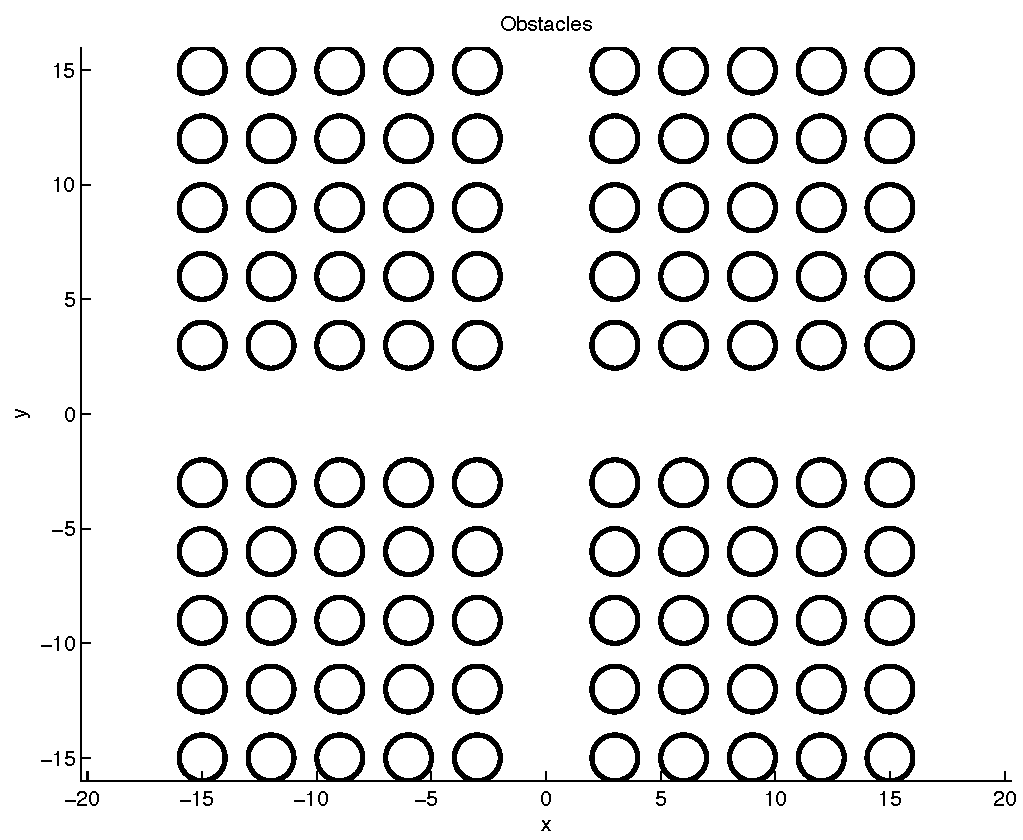
\includegraphics[width=0.45\textwidth]{matlab/fig_WaveguidePenetrable/obstacles.pdf}\label{fig:exwaveguidea}}
\subfigure[Radar cross section]{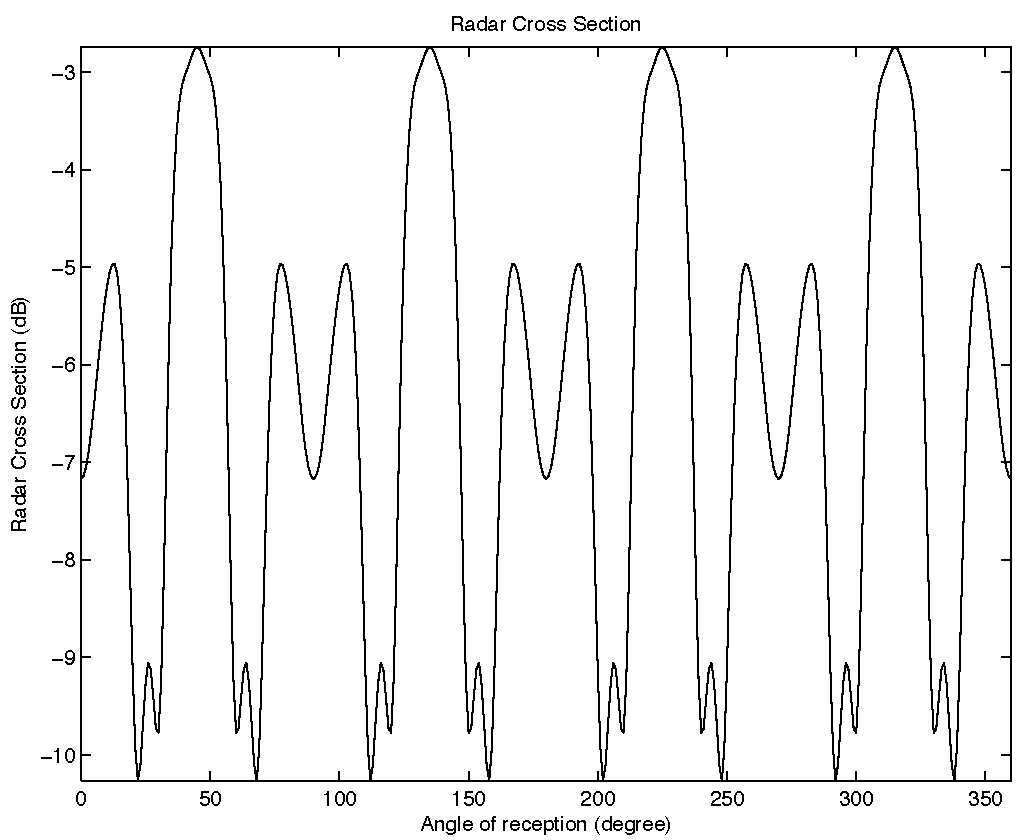
\includegraphics[width=0.45\textwidth]{matlab/fig_WaveguidePenetrable/RCS.pdf}\label{fig:exwaveguideb}}
\subfigure[Absolute value of the total field]{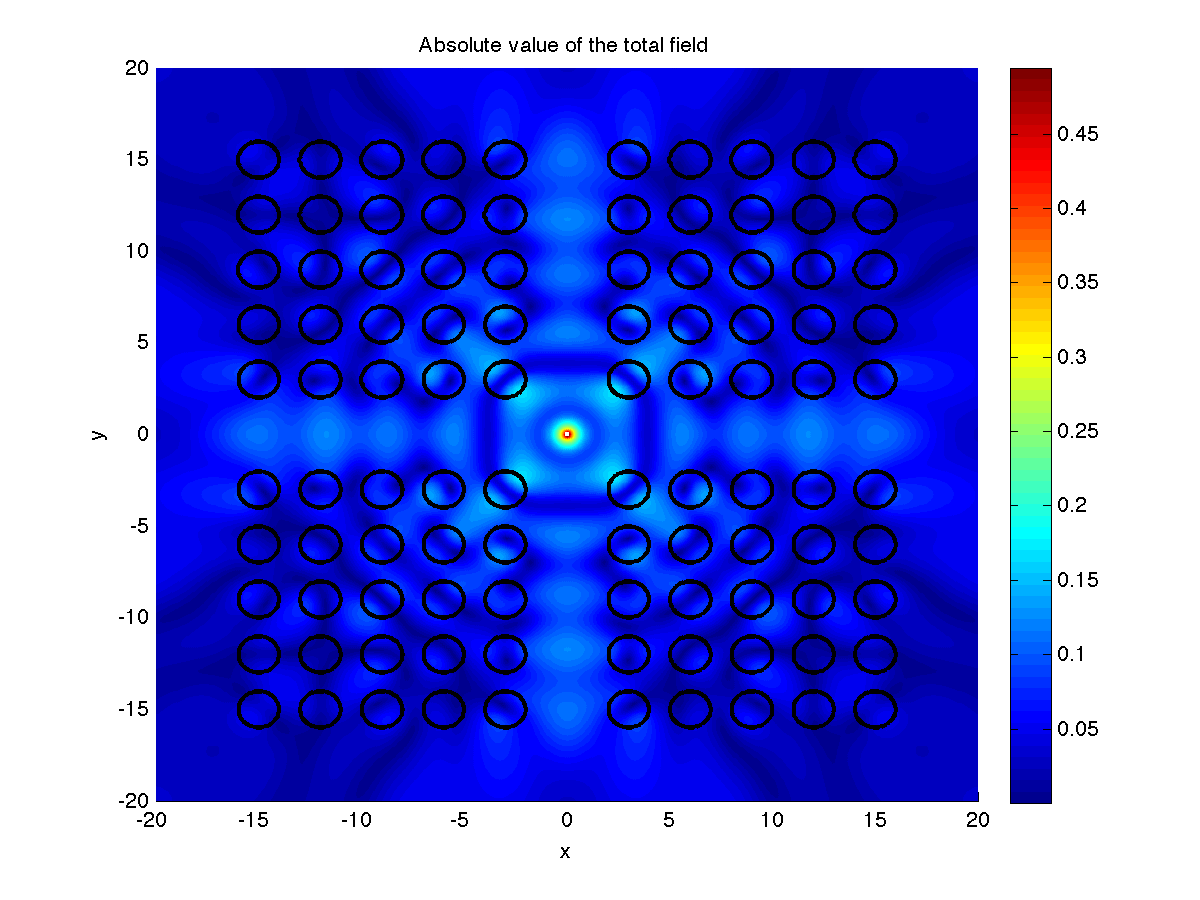
\includegraphics[width=0.45\textwidth]{matlab/fig_WaveguidePenetrable/utot_abs.png}\label{fig:exwaveguided}}
\subfigure[Real part of the total field]{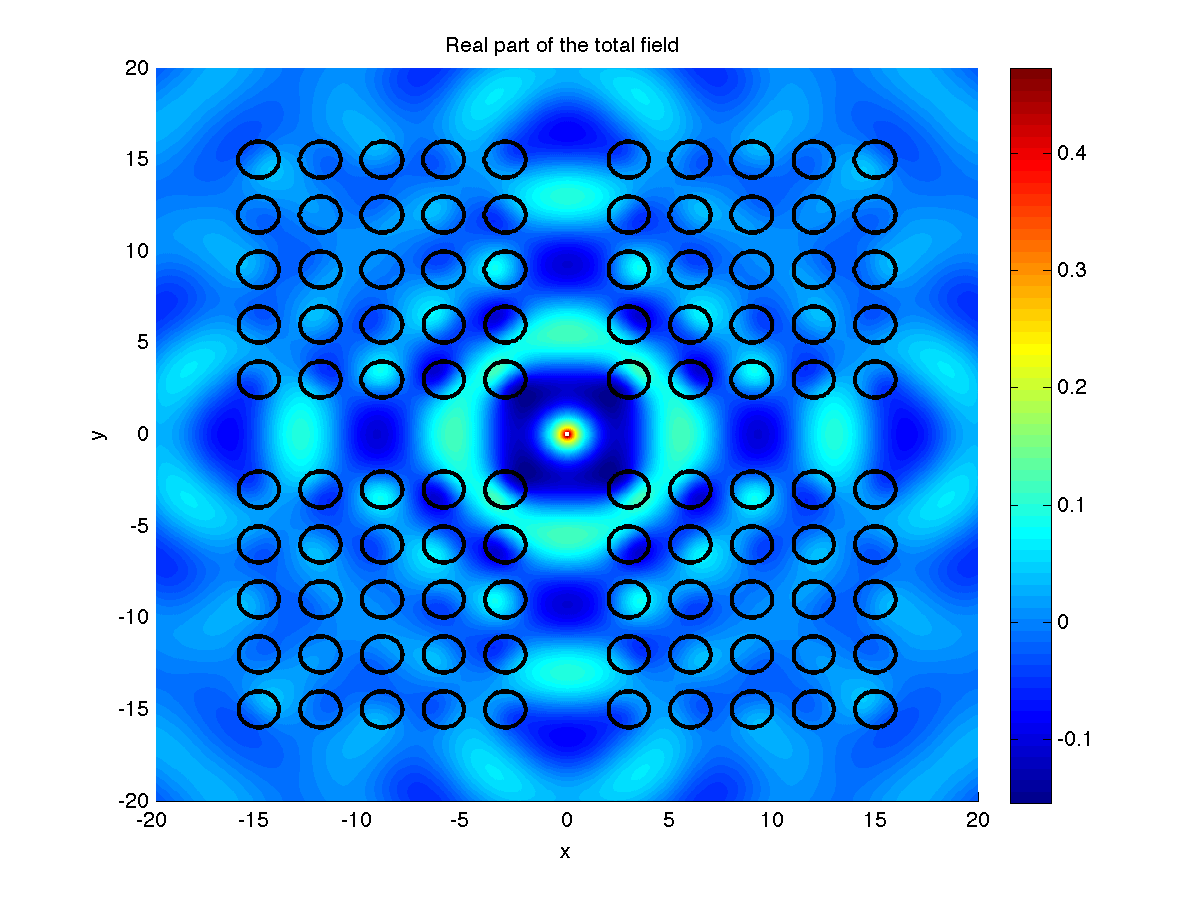
\includegraphics[width=0.45\textwidth]{matlab/fig_WaveguidePenetrable/utot_real.png}\label{fig:exwaveguidee}}
\subfigure[Imaginary part of the total field]{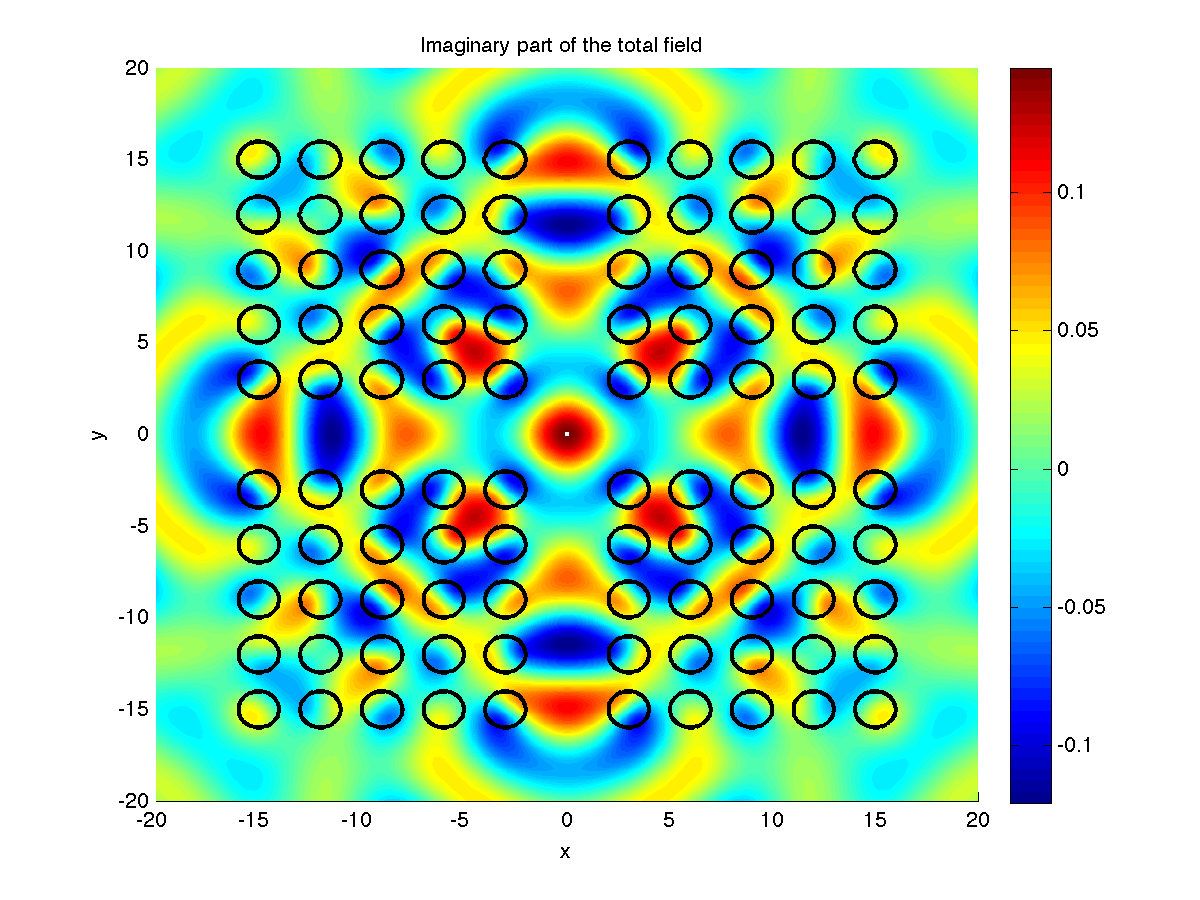
\includegraphics[width=0.45\textwidth]{matlab/fig_WaveguidePenetrable/utot_imag.png}\label{fig:exwaveguidef}}
\caption{Results obtained for a complex geometry of penetrable obstacles with $k=1$ and $k^- =2k$, solved using a single-layer potential representation of the field. The point source is located on $(0,0)$, in the center of the geometry.}
\label{fig:exwaveguide}
\end{figure}




